\documentclass{beamer}

%\usepackage[table]{xcolor}
\mode<presentation> {
  \usetheme{Boadilla}
%  \usetheme{Pittsburgh}
%\usefonttheme[2]{sans}
\renewcommand{\familydefault}{cmss}
%\usepackage{lmodern}
%\usepackage[T1]{fontenc}
%\usepackage{palatino}
%\usepackage{cmbright}
  \setbeamercovered{transparent}
\useinnertheme{rectangles}
}
%\usepackage{normalem}{ulem}
%\usepackage{colortbl, textcomp}
\setbeamercolor{normal text}{fg=black}
\setbeamercolor{structure}{fg= black}
\definecolor{trial}{cmyk}{1,0,0, 0}
\definecolor{trial2}{cmyk}{0.00,0,1, 0}
\definecolor{darkgreen}{rgb}{0,.4, 0.1}
\usepackage{array}
\beamertemplatesolidbackgroundcolor{white}  \setbeamercolor{alerted
text}{fg=red}

\setbeamertemplate{caption}[numbered]\newcounter{mylastframe}

%\usepackage{color}
\usepackage{tikz}
\usetikzlibrary{arrows}
\usepackage{colortbl}
%\usepackage[usenames, dvipsnames]{color}
%\setbeamertemplate{caption}[numbered]\newcounter{mylastframe}c
%\newcolumntype{Y}{\columncolor[cmyk]{0, 0, 1, 0}\raggedright}
%\newcolumntype{C}{\columncolor[cmyk]{1, 0, 0, 0}\raggedright}
%\newcolumntype{G}{\columncolor[rgb]{0, 1, 0}\raggedright}
%\newcolumntype{R}{\columncolor[rgb]{1, 0, 0}\raggedright}

%\begin{beamerboxesrounded}[upper=uppercol,lower=lowercol,shadow=true]{Block}
%$A = B$.
%\end{beamerboxesrounded}}
\renewcommand{\familydefault}{cmss}
%\usepackage[all]{xy}

\usepackage{tikz}
\usepackage{lipsum}

 \newenvironment{changemargin}[3]{%
 \begin{list}{}{%
 \setlength{\topsep}{0pt}%
 \setlength{\leftmargin}{#1}%
 \setlength{\rightmargin}{#2}%
 \setlength{\topmargin}{#3}%
 \setlength{\listparindent}{\parindent}%
 \setlength{\itemindent}{\parindent}%
 \setlength{\parsep}{\parskip}%
 }%
\item[]}{\end{list}}
\usetikzlibrary{arrows}
%\usepackage{palatino}
%\usepackage{eulervm}
\usecolortheme{lily}
\newtheorem{com}{Comment}
\newtheorem{lem} {Lemma}
\newtheorem{prop}{Proposition}
\newtheorem{thm}{Theorem}
\newtheorem{defn}{Definition}
\newtheorem{cor}{Corollary}
\newtheorem{obs}{Observation}
 \numberwithin{equation}{section}
%\usepackage[latin1]{inputenc}
\title[Text as Data] % (optional, nur bei langen Titeln nötig)
{Text as Data}

\author{Justin Grimmer}
\institute[University of Chicago]{Associate Professor\\Department of Political Science \\  University of Chicago}
\vspace{0.3in}


\date{August 23rd, 2017}%[Big Data Workshop]
%\date{\today}



\begin{document}
\begin{frame}
\titlepage
\end{frame}



\begin{frame}
\frametitle{Discovery and Measurement}

What is the research process? (Grimmer, Roberts, and Stewart 2017)

\begin{itemize}
  \item[1)] \alert{Discovery}: a hypothesis or view of the world
  \item[2)] \alert{Measurement} according to some organization
  \item[3)] \alert{Causal Inference}: effect of some intervention
\end{itemize}

Text as data methods assist at each stage of research process

\end{frame}



\begin{frame}

\huge

Measurement


\end{frame}


\begin{frame}

Two approaches to measurement
\begin{itemize}
\item[1)] Use an existing classification scheme to categorize documents
\item[2)] \alert{Simultaneously discover categories and measure prevalence (repurpose discovery methods)}
\end{itemize}

\end{frame}










\begin{frame}
\frametitle{Topic and Mixed Membership Models}

\invisible<6->{\alert{Clustering}\\
 Document $\leadsto$ One Cluster}\\
\invisible<1-5>{\alert{Topic Models} (Mixed Membership) \\
Document $\leadsto$ Many clusters}


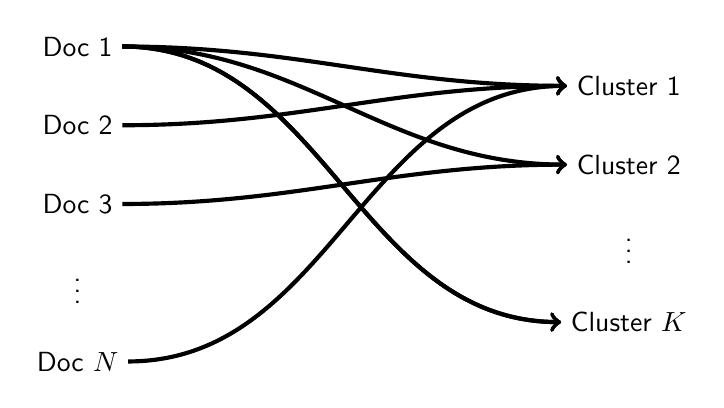
\begin{tikzpicture}

\node (doc1) at (-8,5.5) [] {Doc 1} ;
\node (doc2) at (-8, 4.5) [] {Doc 2} ;
\node (doc3) at (-8, 3.5) [] {Doc 3} ;
\node (doc4) at (-8, 2.5) [] {$\vdots$} ;
\node (doc5) at ( -8, 1.5) [] {Doc $N$} ;


\node (clust1) at (-1, 5) [] {Cluster 1} ;
\node (clust2) at (-1, 4) [] {Cluster 2} ;
\node (clustd) at (-1, 3) [] {$\vdots$} ;
\node (clust4) at (-1, 2) [] {Cluster $K$} ;

\invisible<1,3->{\draw[->, line width = 1.5pt]  (doc1)  to [out=0, in=180] (clust4) ; }
\invisible<1-2,4->{\draw[->, line width = 1.5pt]  (doc2)  to [out=0, in=180] (clust1) ; }
\invisible<1-3,5->{\draw[->, line width = 1.5pt]  (doc3)  to [out=0, in=180] (clust2) ; }
\invisible<1-4,6->{\draw[->, line width = 1.5pt]  (doc5)  to [out=0, in=180] (clust1) ; }

\invisible<1-6>{\draw[->, line width= 1.5pt] (doc1) to [out=0, in =180] (clust1) ;
\draw[->, line width= 1.5pt] (doc1) to [out=0, in =180] (clust2) ;
\draw[->, line width= 1.5pt] (doc1) to [out=0, in =180] (clust4) ;
}


\end{tikzpicture}

\pause \pause \pause \pause \pause \pause

\end{frame}


\begin{frame}
\frametitle{A Statistical Highlighter (With Many Colors) }


\scalebox{0.45}{\includegraphics{WallachHighlighter.png}}

\end{frame}



\begin{frame}
\frametitle{Vanilla Latent Dirichlet Allocation$\leadsto$ Objective Function}

\begin{itemize}
\item[-] Consider document $i$, $(i =1, 2, \hdots, N)$.
\invisible<1>{\item[-] Suppose there are $M_{i}$ total words and $\boldsymbol{x}_{i}$ is an $M_{i} \times 1$ vector, where $x_{im}$ describes the $m^{\text{th}}$ word used in the document$^{*}$.    }
\end{itemize}


\begin{eqnarray}
\invisible<1-6>{\boldsymbol{\theta}_{k} & \sim & \text{Dirichlet}(\boldsymbol{1}) \nonumber }\\
\invisible<1-7>{\alpha_{k} & \sim & \text{Gamma}(\alpha, \beta) \nonumber } \\
\invisible<1-3>{\boldsymbol{\pi}_{i}|\boldsymbol{\alpha} & \sim & \text{Dirichlet}(\boldsymbol{\alpha}) }\nonumber \\
\invisible<1-4>{\boldsymbol{\tau}_{im}| \boldsymbol{\pi}_{i} & \sim & \text{Multinomial}(1, \boldsymbol{\pi}_{i})} \nonumber \\
\invisible<1-5>{x_{im} | \boldsymbol{\theta}_{k}, \tau_{imk}=1 & \sim & \text{Multinomial}(1, \boldsymbol{\theta}_{k}) }\nonumber
\end{eqnarray}


\invisible<1-2, 4->{$^{*}$Notice: this is a different representation than a document-term matrix.  $x_{im}$ is a number that says which of the $J$ words are used.  The difference is for clarity and we'll this representation is closely related to document-term matrix}


\pause \pause \pause \pause \pause \pause \pause
\end{frame}


\begin{frame}
\frametitle{Vanilla Latent Dirichlet Allocation$\leadsto$ Objective Function}

Together the model implies the following posterior:

\begin{small}
\begin{eqnarray}
\invisible<1>{p(\boldsymbol{\pi}, \boldsymbol{T},\boldsymbol{\Theta}, \boldsymbol{\alpha}| \boldsymbol{X}) & \propto & \nonumber p(\boldsymbol{\alpha}) p(\boldsymbol{\pi}| \boldsymbol{\alpha}) p(\boldsymbol{T}| \boldsymbol{\pi}) p(\boldsymbol{X}| \boldsymbol{\theta}, \boldsymbol{T}) \nonumber } \\
\invisible<1-2>{& \propto & p(\boldsymbol{\alpha}) \prod_{i=1}^{N} \left[p(\boldsymbol{\pi}_{i} | \boldsymbol{\alpha}) \prod_{m=1}^{M_{i}} p(\boldsymbol{\tau}_{im}| \boldsymbol{\pi}) p(x_{im}| \boldsymbol{\theta}_{k}, \tau_{imk}=1) \right ] \nonumber }\\
\invisible<1-3>{& \propto & p(\boldsymbol{\alpha}) \prod_{i=1}^{N} \left[\alert<5>{\frac{\Gamma(\sum_{k=1}^{K} \alpha_{k})}{\prod_{k=1}^{K} \Gamma(\alpha_{k}) } \prod_{k=1}^{K} \pi_{ik}^{\alpha_{k}- 1}} \prod_{m=1}^{M}\prod_{k=1}^{K} \left[ \pi_{ik} \alert<6>{\prod_{j=1}^{J} \theta_{jk}^{x_{imj}} }  \right]^{\tau_{ikm}} \right] }\nonumber
\end{eqnarray}

\end{small}

\invisible<1-6>{Optimization:}
\begin{itemize}
\invisible<1-7>{\item[-] Variational Approximation$\leadsto$ Find ``closest" distribution}
\invisible<1-8>{\item[-] Gibbs sampling $\leadsto$ MCMC algorithm to approximate posterior}
\end{itemize}

\invisible<1-9>{\alert{Described in the slides appendix}}
\pause \pause \pause \pause \pause \pause \pause \pause \pause


\end{frame}


\begin{frame}
\frametitle{Running a Topic Model with STM}


{\tt to the STM Code}






\end{frame}


\begin{frame}
\frametitle{Why does this work$\leadsto$ Co-occurrence}


Where's the information for each word's topic? \pause \\

\invisible<1>{Reconsider document-term matrix} \pause

\begin{center}
\invisible<1-2>{\begin{tabular}{ccccc}
\hline
        & $\text{Word}_1$ & $\text{Word}_2$ & $\hdots$ & $\text{Word}_J$ \\
\hline
Doc$_{1}$  & 0   & 1    & $\hdots$ & 0 \\
Doc$_{2}$ & 2 & 0  & $\hdots$ & 3\\
$\vdots$ & $\vdots$ & $\vdots$ & $\ddots$ & $\vdots$ \\
Doc$_{N}$ & 0 & 1 & $\hdots$ & 1 \\
\hline\hline
\end{tabular}} \pause
\end{center}
\invisible<1-3>{Inner product of Documents (rows): $\textbf{Doc}_{i}^{'} \textbf{Doc}_{l} $} \pause \\
\vspace{0.1in}
\invisible<1-4>{Inner product of Terms (columns): $\textbf{Word}_j^{'} \textbf{Word}_k$ } \pause \\
\invisible<1-5>{\alert{Allows}: measure of correlation of term usage across documents (heuristically: partition words, based on usage in documents)} \pause \\
\invisible<1-6>{\alert{Latent Semantic Analysis}:  Reduce information in matrix using linear algebra (provides similar results, difficult to generalize)} \pause \\
\invisible<1-7>{\alert{Biclustering}: Models that partition documents and words simultaneously}


\end{frame}


\begin{frame}
\frametitle{Why does this work$\leadsto$ Co-occurrence logic (h/t Colorado Reed Tutorial)}

\begin{eqnarray}
\only<1>{p(\boldsymbol{\pi}, \boldsymbol{T},\boldsymbol{\Theta}, \boldsymbol{\alpha}| \boldsymbol{X}) & \propto & \nonumber p(\boldsymbol{\alpha}) p(\boldsymbol{\pi}| \boldsymbol{\alpha}) p(\boldsymbol{T}| \boldsymbol{\pi}) p(\boldsymbol{X}| \boldsymbol{\theta}, \boldsymbol{T}) \nonumber  }
\only<2>{p(\boldsymbol{\pi}, \boldsymbol{T},\boldsymbol{\Theta}, \boldsymbol{\alpha}| \boldsymbol{X}) & \propto & \nonumber p(\boldsymbol{\alpha}) p(\boldsymbol{\pi}| \boldsymbol{\alpha}) p(\boldsymbol{T}| \boldsymbol{\pi}) \underbrace{p(\boldsymbol{X}| \boldsymbol{\theta}, \boldsymbol{T})}_{1} \nonumber  }
\only<3>{p(\boldsymbol{\pi}, \boldsymbol{T},\boldsymbol{\Theta}, \boldsymbol{\alpha}| \boldsymbol{X}) & \propto & \nonumber p(\boldsymbol{\alpha}) p(\boldsymbol{\pi}| \boldsymbol{\alpha}) \underbrace{p(\boldsymbol{T}| \boldsymbol{\pi})}_{2} \underbrace{p(\boldsymbol{X}| \boldsymbol{\theta}, \boldsymbol{T})}_{1} \nonumber  }
\only<4>{p(\boldsymbol{\pi}, \boldsymbol{T},\boldsymbol{\Theta}, \boldsymbol{\alpha}| \boldsymbol{X}) & \propto & \nonumber p(\boldsymbol{\alpha}) \underbrace{p(\boldsymbol{\pi}| \boldsymbol{\alpha})}_{3} \underbrace{p(\boldsymbol{T}| \boldsymbol{\pi})}_{2} \underbrace{p(\boldsymbol{X}| \boldsymbol{\theta}, \boldsymbol{T})}_{1} \nonumber  }
\end{eqnarray}

\begin{itemize}
\invisible<1>{\item[1)] $\boldsymbol{\theta} \leadsto$ Greater weight on terms that occur together}
\invisible<1-2>{\item[2)] $\boldsymbol{\pi} \leadsto$ Greater weight on indicators that appear more regularly}
\invisible<1-3>{\item[3)] $\boldsymbol{\alpha}\leadsto$ Emphasis on $\boldsymbol{\pi}$ with greater weight}
\end{itemize}

\pause \pause \pause


\end{frame}







\begin{frame}
\frametitle{Validation$\leadsto$ Topic Intrusion}

Wednesday$\leadsto$ discussed several validations

\begin{itemize}
\item[-] Labeling paragraphs
\begin{itemize}
\item[-] Identify separating words automatically
\item[-] Label topics manually (read!)
\end{itemize}
\item[-] Statistical methods
\begin{itemize}
\item[1)] Entropy
\item[2)] Exclusivity
\item[3)] Cohesiveness
\end{itemize}
\item[-] Experiment Based Methods
\begin{itemize}
\item[-] Word intrusion$\leadsto$ topic validity
\item[-] \alert{Topic intrusion}$\leadsto$ model fit
\end{itemize}

\end{itemize}



\end{frame}


\begin{frame}
\frametitle{Validation$\leadsto$ Topic Intrusion}


\begin{itemize}
\item[1)] Ask research assistant to read paragraph
\item[2)] Construct experiment
\begin{itemize}
\item[-] For the document, select top three topics
\item[-] Select a fourth topic
\item[-] Show participant, ask her/him to identify intruder
\end{itemize}

Higher identification$\leadsto$ topics are a better model of text


\end{itemize}

\end{frame}




\begin{frame}
\frametitle{Example 1: Japanese Campaign Manifestos (Catalinac 2011)}


\begin{itemize}
\item[-] Why is Japan revising its constitution?
\item[-] \alert{IR} question: why is Japan now willing to engage militaristic foreign action?
\item[-] \alert{One explanation}: election reform in 1993, changed electoral incentives
\item[-] To answer well: characterize campaigns across 50 + years
\begin{itemize}
\item[-] \alert{That sounds hard}
\item[-] \alert{That sounds impossible}
\end{itemize}
\item[-] Determined (relentless) data collection
\item[-] Latent Dirichlet Allocation (on japanese texts)
\end{itemize}


\end{frame}



\begin{frame}
\frametitle{Example 1: Japanese Campaign Manifestos (Catalinac 2011) }


\only<1-3, 5->{
Japanese Elections: \pause
\begin{itemize}
\invisible<1>{\item[-] Election Administration Commission runs elections $\rightarrow$ district level} \pause
\invisible<1-2>{\item[-] Required to submit manifestos for all candidates to National Diet} \pause
\invisible<1-4>{\item[-] Collected from 1950- 2009} \pause
\begin{itemize}
\invisible<1-5>{\item[-] Available only at district level} \pause
\invisible<1-6>{\item[-] \alert{Until}: 2009 national library made texts available on microfilm } \pause
\end{itemize}
\invisible<1-7>{\item[-] Collected from microfilm, hand transcribed (no OCR worked), used a variety of techniques to create a TDM } \pause
\invisible<1-8>{\item[-] \alert{Harder for Japanese} }
\end{itemize}
}


\only<4>{
Typical Manifesto:
\scalebox{0.45}{\includegraphics{Tokyo1.pdf}}}\pause


\end{frame}

\begin{frame}
\frametitle{Example 1:  Japanese Campaign Manifestos (Catalinac 2014)}

\begin{itemize}
\item[-] Applies Vanilla LDA (using R Code )
\item[-] Output: topics (with Japanese characters)
\end{itemize}

\end{frame}


\begin{frame}
\frametitle{Example 1: Japanese Campaign Manifestos (Catalinac 2011)}

\scalebox{0.3}{\includegraphics{Topics.png} }

\end{frame}


\begin{frame}
\frametitle{Example 1: Japanese Campaign Manifestos (Catalinac 2011)}

\only<1>{\scalebox{0.4}{\includegraphics{Pork.pdf} }}
\only<2>{\scalebox{0.4}{\includegraphics{NatSecurity.pdf}}}

\end{frame}


\begin{frame}

\scalebox{0.5}{\includegraphics{Cover1.jpg}}


\end{frame}




\begin{frame}
\frametitle{Example 2: Automated Literature Reviews}

\alert{Recall}: literature reviews are hard to conduct\\
\alert{LDA}: developed (in part) to help structure {\tt JSTOR} database\\
Use {\tt JSTOR}'s research service to obtain data to analyze\\
\alert{Question:} How do scholars use classic text: \alert{Home Style}\\
Analysis: all articles that cite \alert{Home Style} in JSTOR's data\\

\end{frame}





\begin{frame}
\frametitle{Example 2: Automated Literature Reviews}

Output: topic estimates
\begin{itemize}
\item[-] Obtain $\log \theta_k$ from model
\item[-] One method to summarize a topic:
\begin{itemize}
\item[-] $\exp(\log \theta_k) $ (select 10-20 biggest words)
\item[-] $\exp(\log \theta_k) - \text{Average}_{j\neq k} \exp(\log \theta_j)$ (select 10-20 biggest words)
\end{itemize}
\end{itemize}


\end{frame}

\begin{frame}
\frametitle{Example 2: Automated Literature Reviews}
Example topics:
\small
\begin{tabular}{lll}
\hline\hline
Label & Stems & Proportion of Docs \\
\hline
Life Style & member,district,attent,congress,time,cohort,retir & 0.03  \\
Comp.Home & constitu,mp,member,parti,role,local,british &  0.02  \\
Casework & casework,district,constitu,variabl,staff,congression,fiorina & 0.03\\
Votes & vote,variabl,model,estim,measur,legisl,constitu & 0.04 \\
Id. Shirk & ideolog,vote,shirk,constitu,parti,senat,voter & 0.03\\
C. letters & mail,govern, activ,respond,commun,offic &  0.02\\
\hline
\hline
\end{tabular}


\end{frame}

\begin{frame}
\frametitle{Example Document}


\only<1>{Wawro (2001) ``A Panel Probit Analysis of Campaign Contributions and Roll Call Votes"
\scalebox{0.4}{\includegraphics{Wawro.pdf}} }
\only<2>{Bender (1996) ``Legislator Voting and Shirking  A Critical Review of the Literature"
\scalebox{0.4}{\includegraphics{Bender.pdf}}}
\only<3>{Parker (1980) ``Cycles in Congressional District Attention"
\scalebox{0.4}{\includegraphics{Parker.pdf}}}
\only<4>{Shepsle (1985) ``Policy Consequences of Government by Congressional Subcommittees"
\scalebox{0.4}{\includegraphics{Shepsle.pdf}} }


\end{frame}




\begin{frame}
\frametitle{History of Home Style}



\begin{center}
\only<1>{\scalebox{0.4}{\includegraphics{Home1.pdf}} }
\only<2>{\scalebox{0.4}{\includegraphics{Home2.pdf}} }
\only<3>{\scalebox{0.4}{\includegraphics{Home3.pdf}} }
\only<4>{\scalebox{0.4}{\includegraphics{Vote1.pdf}} }
\only<5>{\scalebox{0.4}{\includegraphics{Vote2.pdf}} }
\only<6>{\scalebox{0.4}{\includegraphics{Vote3.pdf}} }
\end{center}


\end{frame}



\begin{frame}

\begin{center}
\scalebox{0.1}{\includegraphics{Cover2.jpg}}
\end{center}

\end{frame}


\begin{frame}

\begin{center}
What legislators claim (Grimmer, Westwood, Messing 2014) \pause \invisible<1>{$\leadsto$ LDA credit claiming press releases}

\begin{footnotesize}
\begin{tabular}{lll}
\hline\hline
\invisible<1>{Labels & Key Words & Proportion}  \\
\hline
\invisible<1-2>{Requested appropriations&bill,funding,house,million,appropriations&0.08}   \\
\invisible<1-4>{Fire department grants&fire,grant,department,program,firefighters&0.08 } \\
\invisible<1-6>{Stimulus&recovery,funding,jobs,information, act, &0.06}   \\
\invisible<1-7>{Transportation&transportation,project,airport,transit,million&0.06}  \\
\end{tabular}
\end{footnotesize}
\end{center}


\invisible<1-2>{\only<1-3>{
``Dave Camp announced today that he was able to secure \$2.5 million for widening
M-72 from US-31 easterly 7.2 miles to Old M-72.  \alert{The
bill will now head to the Senate for consideration...We have two more hurdles to clear to make sure the money is in the bill when it
hits the President's desk: a vote in the Senate and a conference committee}" (Camp, 2005)}}


\only<4>{``Congressman Doc Hastings has boosted federal funding for work on the Columbia Basin water supply for next year. Hastings has added \$400,000 for work on the Odessa Subaquifer, which when combined with the funding in the President's budget request, totals \$1 million for Fiscal Year 2009"...``\alert{Hastings' funding for the Odessa Subaquifer and Potholes Reservoir was included in the Fiscal Year 2009 Energy and Water Appropriations bill which was approved today by the full House Appropriations Committee. (Hastings, 2008)}"}



\only<5>{``Maurice Hinchey (D-NY) today \alert{announced} that the West Endicott Fire Company has been awarded a \$17,051 federal grant to purchase approximately 10 sets of protective clothing, as well as radio equipment and air packs for its volunteer firefighters" (Hinchey, 2008) }


\only<6>{``Congressman Pete Visclosky today \alert{announced} that the Crown Point Fire Department
will receive a \$16,550 Department of Homeland Security (DHS) grant to purchase a
modular portable video system" (Visclosky, 2008)}



\pause\pause \pause \pause \pause \pause







\end{frame}





\begin{frame}
\frametitle{Correlated Topic Models}

Dirichlet distribution$\leadsto$ Assumes negative covariance between topics\\
\alert{Logistic Normal Distribution}$\leadsto$ Allows some positive covariance between topics\\

\begin{eqnarray}
\boldsymbol{\theta}_{k} & \sim & \text{Dirichlet}(\boldsymbol{1}) \nonumber \\
\boldsymbol{\eta}_{i}| \boldsymbol{\mu}, \boldsymbol{\Sigma} & \sim & \text{Multivariate Normal}(\boldsymbol{\mu}, \boldsymbol{\Sigma}) \nonumber \\
\boldsymbol{\pi}_{i}  & = & \frac{\exp\left(\boldsymbol{\eta}_{i}\right)}{\sum_{k=1}^{K} \exp\left(\eta_{ik}\right)} \nonumber \\
\boldsymbol{\tau}_{im} | \boldsymbol{\pi}_{i} & \sim & \text{Multinomial}(1, \boldsymbol{\pi}_{i}) \nonumber \\
x_{im} | \boldsymbol{\theta}_{k}, \tau_{imk} = 1 & \sim & \text{Multinomial}(1, \boldsymbol{\theta}_{k}) \nonumber
\end{eqnarray}



\end{frame}




\begin{frame}
\frametitle{LDA Revisited}


\only<1>{\begin{eqnarray}
\boldsymbol{\theta}_{k} & \sim & \text{Dirichlet}(\boldsymbol{1}) \nonumber \\
\boldsymbol{\pi}_{i}|\boldsymbol{\alpha} & \sim &  \text{Dirichlet}(\boldsymbol{\alpha}) \nonumber \\
\boldsymbol{\tau}_{im}| \boldsymbol{\pi}_{i} & \sim & \text{Multinomial}(1, \boldsymbol{\pi}_{i}) \nonumber \\
x_{im} | \boldsymbol{\theta}_{k}, \tau_{imk} = 1 & \sim & \text{Multinomial}(1, \boldsymbol{\theta}_{k}) \nonumber
\end{eqnarray}}

\only<2>{\begin{eqnarray}
\textbf{Unigram Model}_{k} & \sim & \text{Dirichlet}(\boldsymbol{1}) \nonumber \\
\textbf{Doc. Prop}_{i} & \sim & \text{Dirichlet}(\textbf{Pop. Proportion}) \nonumber \\
\textbf{Word Topic}_{im} & \sim & \text{Multinomial}(1, \textbf{Doc. Prop}_{i}) \nonumber \\
\text{Word}_{im} & \sim & \text{Multinomial}(1, \textbf{Unigram Model}_{k}) \nonumber
\end{eqnarray}}







\end{frame}



\begin{frame}
\frametitle{A General Hierarchical Structure}

LDA:
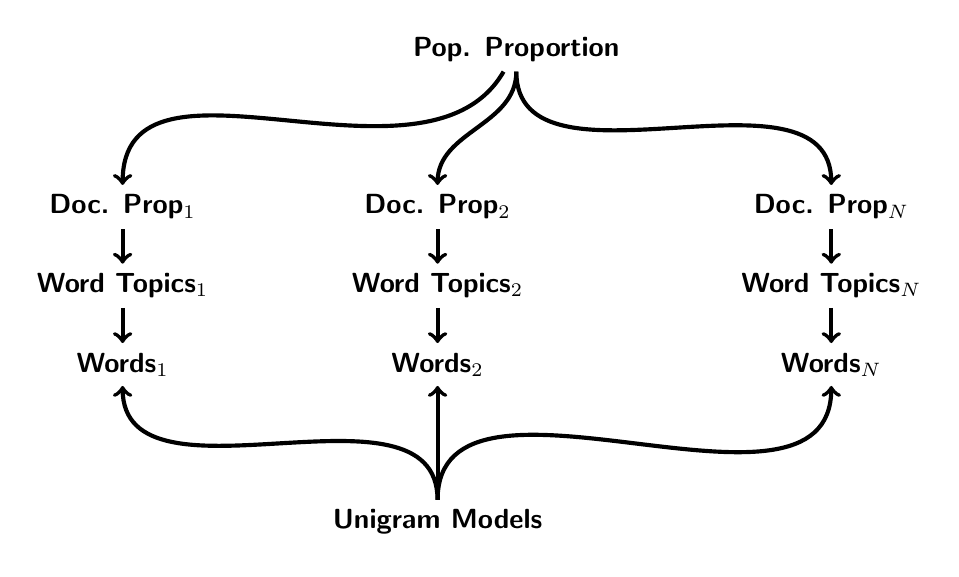
\begin{tikzpicture}

\node (col) at (0, 10) [] {\textbf{Pop. Proportion}} ;

\invisible<1>{



\node (doc1) at (-5, 8) [] {\textbf{Doc. Prop}$_{1}$} ;
\node (doc2) at (-1, 8) [] {\textbf{Doc. Prop}$_{2}$} ;
\node (dots) at ( 2, 8) [] {$\hdots$} ;
\node (docN) at (4, 8) [] {\textbf{Doc. Prop}$_{N}$} ;

\draw[->, line width=1.5pt] (col) to [out=240, in = 90] (doc1);
\draw[->, line width=1.5pt] (col) to [out=270, in = 90] (doc2);
\draw[->, line width=1.5pt] (col) to [out=270, in = 90] (docN);

}

\invisible<1-2>{


\node (word11) at (-5, 7) [] {\textbf{Word Topics}$_{1}$} ;
\node (word22) at (-1, 7) [] {\textbf{Word Topics}$_{2}$} ;
\node (wordnn) at (4, 7) [] {\textbf{Word Topics}$_{N}$ } ;

\draw[->, line width=1.5pt] (doc1) to [out=270, in=90] (word11) ;
\draw[->, line width=1.5pt] (doc2) to [out=270, in=90] (word22) ;
\draw[->, line width=1.5pt] (docN) to [out=270, in=90] (wordnn) ;




}



\invisible<1-3>{

\node (wordaa) at (-5, 6) [] {\textbf{Words}$_{1}$} ;
\node (wordbb) at (-1, 6) [] {\textbf{Words}$_{2}$} ;
\node (wordcc) at (4, 6) [] {\textbf{Words}$_{N}$ } ;


\draw[->, line width = 1.5pt] (word11) to [out = 270, in = 90] (wordaa);
\draw[->, line width = 1.5pt] (word22) to [out = 270, in = 90] (wordbb);
\draw[->, line width = 1.5pt] (wordnn) to [out = 270, in = 90] (wordcc);

\node (topics) at (-1, 4) [] {$\textbf{Unigram Models}$} ;



\draw[->, line width = 1.5pt] (topics) to [out = 90, in = 270] (wordaa);
\draw[->, line width = 1.5pt] (topics) to [out = 90, in = 270] (wordbb);
\draw[->, line width = 1.5pt] (topics) to [out = 90, in = 270] (wordcc);



}


\end{tikzpicture}


\pause \pause \pause

\end{frame}



\begin{frame}
\frametitle{A General Hierarchical Structure}

Dynamic Topic Model (Quinn et al 2010)
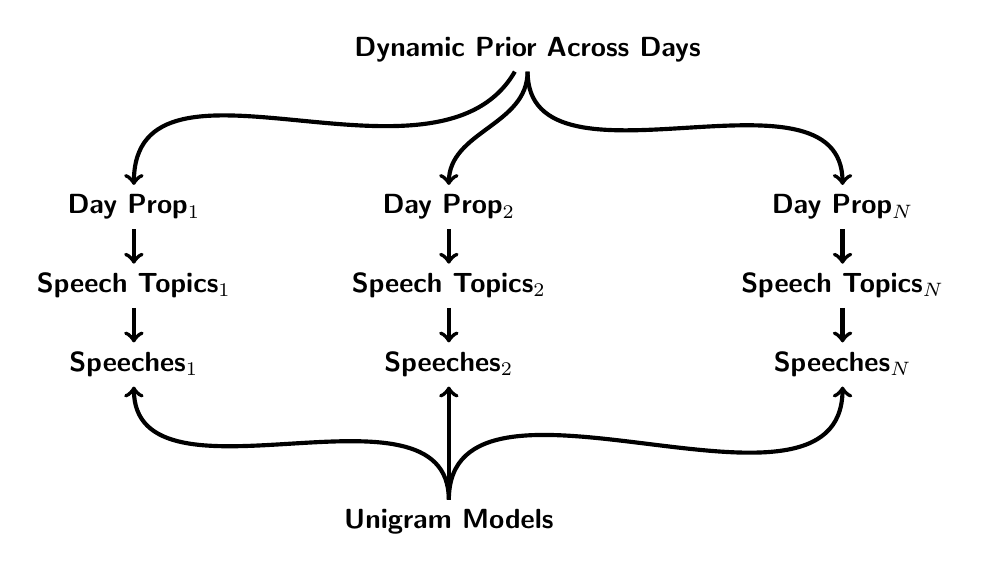
\begin{tikzpicture}

\node (col) at (0, 10) [] {\textbf{Dynamic Prior Across Days}} ;

\invisible<1>{



\node (doc1) at (-5, 8) [] {\textbf{Day Prop}$_{1}$} ;
\node (doc2) at (-1, 8) [] {\textbf{Day Prop}$_{2}$} ;
\node (dots) at ( 2, 8) [] {$\hdots$} ;
\node (docN) at (4, 8) [] {\textbf{Day Prop}$_{N}$} ;

\draw[->, line width=1.5pt] (col) to [out=240, in = 90] (doc1);
\draw[->, line width=1.5pt] (col) to [out=270, in = 90] (doc2);
\draw[->, line width=1.5pt] (col) to [out=270, in = 90] (docN);

}

\invisible<1-2>{


\node (word11) at (-5, 7) [] {\textbf{Speech Topics}$_{1}$} ;
\node (word22) at (-1, 7) [] {\textbf{Speech Topics}$_{2}$} ;
\node (wordnn) at (4, 7) [] {\textbf{Speech Topics}$_{N}$ } ;

\draw[->, line width=1.5pt] (doc1) to [out=270, in=90] (word11) ;
\draw[->, line width=1.5pt] (doc2) to [out=270, in=90] (word22) ;
\draw[->, line width=1.5pt] (docN) to [out=270, in=90] (wordnn) ;




}



\invisible<1-3>{

\node (wordaa) at (-5, 6) [] {\textbf{Speeches}$_{1}$} ;
\node (wordbb) at (-1, 6) [] {\textbf{Speeches}$_{2}$} ;
\node (wordcc) at (4, 6) [] {\textbf{Speeches}$_{N}$ } ;


\draw[->, line width = 1.5pt] (word11) to [out = 270, in = 90] (wordaa);
\draw[->, line width = 1.5pt] (word22) to [out = 270, in = 90] (wordbb);
\draw[->, line width = 1.5pt] (wordnn) to [out = 270, in = 90] (wordcc);

\node (topics) at (-1, 4) [] {$\textbf{Unigram Models}$} ;



\draw[->, line width = 1.5pt] (topics) to [out = 90, in = 270] (wordaa);
\draw[->, line width = 1.5pt] (topics) to [out = 90, in = 270] (wordbb);
\draw[->, line width = 1.5pt] (topics) to [out = 90, in = 270] (wordcc);



}


\end{tikzpicture}


\pause \pause \pause

\end{frame}




\begin{frame}
\frametitle{A General Hierarchical Structure}

Expressed Agenda Model (Grimmer 2010)
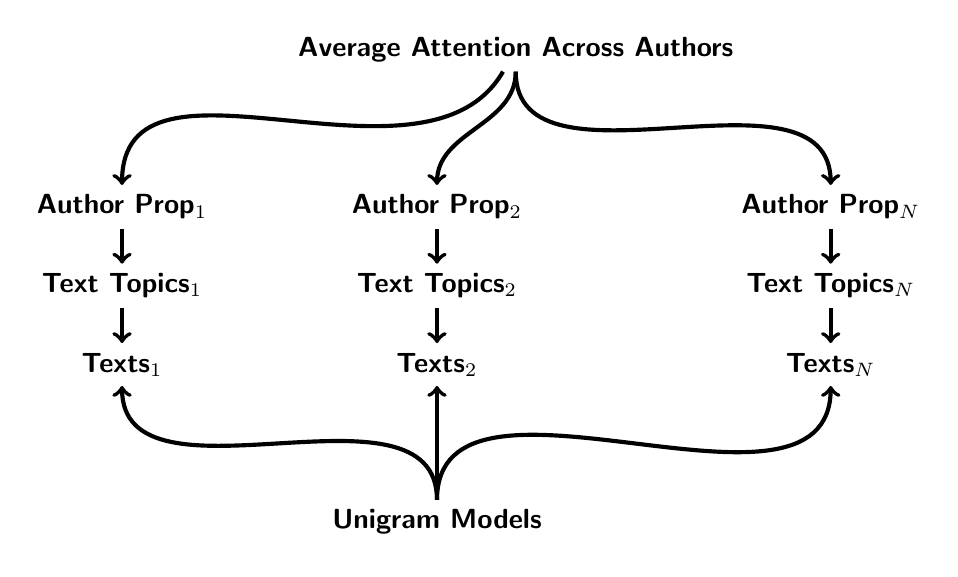
\begin{tikzpicture}

\node (col) at (0, 10) [] {\textbf{Average Attention Across Authors}} ;

\invisible<1>{



\node (doc1) at (-5, 8) [] {\textbf{Author Prop}$_{1}$} ;
\node (doc2) at (-1, 8) [] {\textbf{Author Prop}$_{2}$} ;
\node (dots) at ( 2, 8) [] {$\hdots$} ;
\node (docN) at (4, 8) [] {\textbf{Author Prop}$_{N}$} ;

\draw[->, line width=1.5pt] (col) to [out=240, in = 90] (doc1);
\draw[->, line width=1.5pt] (col) to [out=270, in = 90] (doc2);
\draw[->, line width=1.5pt] (col) to [out=270, in = 90] (docN);

}

\invisible<1-2>{


\node (word11) at (-5, 7) [] {\textbf{Text Topics}$_{1}$} ;
\node (word22) at (-1, 7) [] {\textbf{Text Topics}$_{2}$} ;
\node (wordnn) at (4, 7) [] {\textbf{Text Topics}$_{N}$ } ;

\draw[->, line width=1.5pt] (doc1) to [out=270, in=90] (word11) ;
\draw[->, line width=1.5pt] (doc2) to [out=270, in=90] (word22) ;
\draw[->, line width=1.5pt] (docN) to [out=270, in=90] (wordnn) ;




}



\invisible<1-3>{

\node (wordaa) at (-5, 6) [] {\textbf{Texts}$_{1}$} ;
\node (wordbb) at (-1, 6) [] {\textbf{Texts}$_{2}$} ;
\node (wordcc) at (4, 6) [] {\textbf{Texts}$_{N}$ } ;


\draw[->, line width = 1.5pt] (word11) to [out = 270, in = 90] (wordaa);
\draw[->, line width = 1.5pt] (word22) to [out = 270, in = 90] (wordbb);
\draw[->, line width = 1.5pt] (wordnn) to [out = 270, in = 90] (wordcc);

\node (topics) at (-1, 4) [] {$\textbf{Unigram Models}$} ;



\draw[->, line width = 1.5pt] (topics) to [out = 90, in = 270] (wordaa);
\draw[->, line width = 1.5pt] (topics) to [out = 90, in = 270] (wordbb);
\draw[->, line width = 1.5pt] (topics) to [out = 90, in = 270] (wordcc);



}


\end{tikzpicture}


\pause \pause \pause

\end{frame}


\begin{frame}
\frametitle{A General Hierarchical Structure}

Structural Topic Model (Roberts, Stewart, Airoldi 2014)
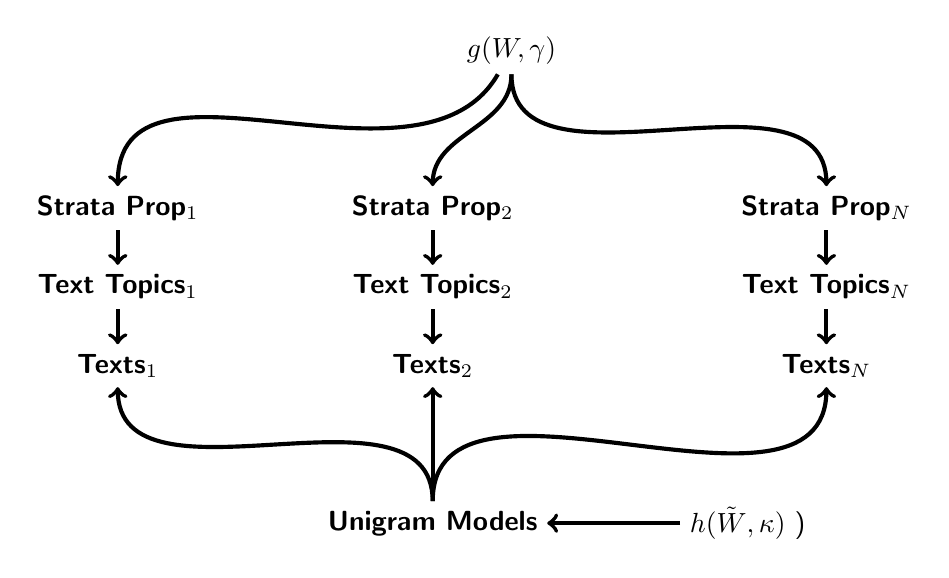
\begin{tikzpicture}

\node (col) at (0, 10) [] {$g(\boldsymbol{W}, \boldsymbol{\gamma}) $} ;

\invisible<1>{



\node (doc1) at (-5, 8) [] {\textbf{Strata Prop}$_{1}$} ;
\node (doc2) at (-1, 8) [] {\textbf{Strata Prop}$_{2}$} ;
\node (dots) at ( 2, 8) [] {$\hdots$} ;
\node (docN) at (4, 8) [] {\textbf{Strata Prop}$_{N}$} ;

\draw[->, line width=1.5pt] (col) to [out=240, in = 90] (doc1);
\draw[->, line width=1.5pt] (col) to [out=270, in = 90] (doc2);
\draw[->, line width=1.5pt] (col) to [out=270, in = 90] (docN);

}

\invisible<1-2>{


\node (word11) at (-5, 7) [] {\textbf{Text Topics}$_{1}$} ;
\node (word22) at (-1, 7) [] {\textbf{Text Topics}$_{2}$} ;
\node (wordnn) at (4, 7) [] {\textbf{Text Topics}$_{N}$ } ;

\draw[->, line width=1.5pt] (doc1) to [out=270, in=90] (word11) ;
\draw[->, line width=1.5pt] (doc2) to [out=270, in=90] (word22) ;
\draw[->, line width=1.5pt] (docN) to [out=270, in=90] (wordnn) ;




}



\invisible<1-3>{

\node (wordaa) at (-5, 6) [] {\textbf{Texts}$_{1}$} ;
\node (wordbb) at (-1, 6) [] {\textbf{Texts}$_{2}$} ;
\node (wordcc) at (4, 6) [] {\textbf{Texts}$_{N}$ } ;


\draw[->, line width = 1.5pt] (word11) to [out = 270, in = 90] (wordaa);
\draw[->, line width = 1.5pt] (word22) to [out = 270, in = 90] (wordbb);
\draw[->, line width = 1.5pt] (wordnn) to [out = 270, in = 90] (wordcc);

\node (topics) at (-1, 4) [] {$\textbf{Unigram Models}$} ;



\draw[->, line width = 1.5pt] (topics) to [out = 90, in = 270] (wordaa);
\draw[->, line width = 1.5pt] (topics) to [out = 90, in = 270] (wordbb);
\draw[->, line width = 1.5pt] (topics) to [out = 90, in = 270] (wordcc);



}

\invisible<1-4>{
\node (reg) at (3, 4) [] {$h(\tilde{\boldsymbol{W}}, \boldsymbol{\kappa})$ )};

\draw[->, line width = 1.5pt] (reg) to [out = 180, in = 0] (topics);

}
\end{tikzpicture}


\pause \pause \pause \pause

\end{frame}


\begin{frame}
\frametitle{A General Hierarchical Structure}

Conditioning on Unknown Covariates$\leadsto$ levels of mixtures at proportions (Grimmer 2013; Wallach 2008)
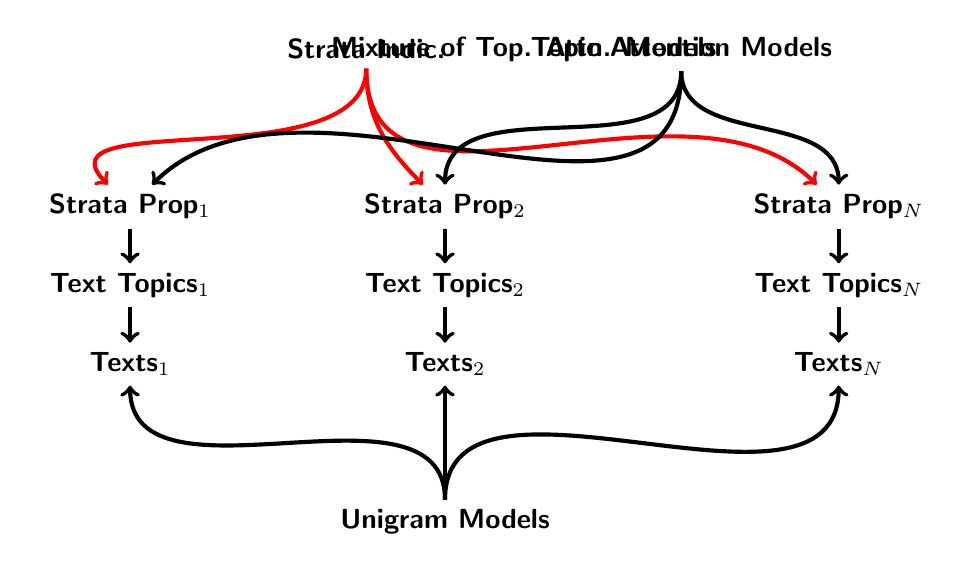
\begin{tikzpicture}

\only<1>{\node (col_on) at (0, 10)[] {\textbf{Mixture of Top. Attn. Models}} ; }

\invisible<1>{\node (col1) at (-2, 10) [] {\textbf{Strata Indic.} } ;
\node (col) at (2, 10) [] {\textbf{Topic Attention Models} }  ; }

\invisible<1-2>{



\node (doc1) at (-5, 8) [] {\textbf{Strata Prop}$_{1}$} ;
\node (doc2) at (-1, 8) [] {\textbf{Strata Prop}$_{2}$} ;
\node (dots) at ( 2, 8) [] {$\hdots$} ;
\node (docN) at (4, 8) [] {\textbf{Strata Prop}$_{N}$} ;


\draw[->, line width=1.5pt, red] (col1) to [out=270, in = 135] (doc1);
\draw[->, line width=1.5pt, red] (col1) to [out=270, in = 135] (doc2);
\draw[->, line width=1.5pt, red] (col1) to [out=270, in = 135] (docN);
}

\invisible<1-3>{

\draw[->, line width=1.5pt] (col) to [out=270, in = 45] (doc1);
\draw[->, line width=1.5pt] (col) to [out=270, in = 90] (doc2);
\draw[->, line width=1.5pt] (col) to [out=270, in = 90] (docN);




}

\invisible<1-4>{


\node (word11) at (-5, 7) [] {\textbf{Text Topics}$_{1}$} ;
\node (word22) at (-1, 7) [] {\textbf{Text Topics}$_{2}$} ;
\node (wordnn) at (4, 7) [] {\textbf{Text Topics}$_{N}$ } ;

\draw[->, line width=1.5pt] (doc1) to [out=270, in=90] (word11) ;
\draw[->, line width=1.5pt] (doc2) to [out=270, in=90] (word22) ;
\draw[->, line width=1.5pt] (docN) to [out=270, in=90] (wordnn) ;




}



\invisible<1-5>{

\node (wordaa) at (-5, 6) [] {\textbf{Texts}$_{1}$} ;
\node (wordbb) at (-1, 6) [] {\textbf{Texts}$_{2}$} ;
\node (wordcc) at (4, 6) [] {\textbf{Texts}$_{N}$ } ;


\draw[->, line width = 1.5pt] (word11) to [out = 270, in = 90] (wordaa);
\draw[->, line width = 1.5pt] (word22) to [out = 270, in = 90] (wordbb);
\draw[->, line width = 1.5pt] (wordnn) to [out = 270, in = 90] (wordcc);

\node (topics) at (-1, 4) [] {$\textbf{Unigram Models}$} ;



\draw[->, line width = 1.5pt] (topics) to [out = 90, in = 270] (wordaa);
\draw[->, line width = 1.5pt] (topics) to [out = 90, in = 270] (wordbb);
\draw[->, line width = 1.5pt] (topics) to [out = 90, in = 270] (wordcc);



}


\end{tikzpicture}


\pause \pause \pause \pause \pause

\end{frame}



\begin{frame}
\frametitle{A General Hierarchical Structure}

Conditioning on Unknown Covariates for Topics$\leadsto$ hierarchy of topics (Li and McCallum 2006; Blaydes, Grimmer, and McQueen 2017)
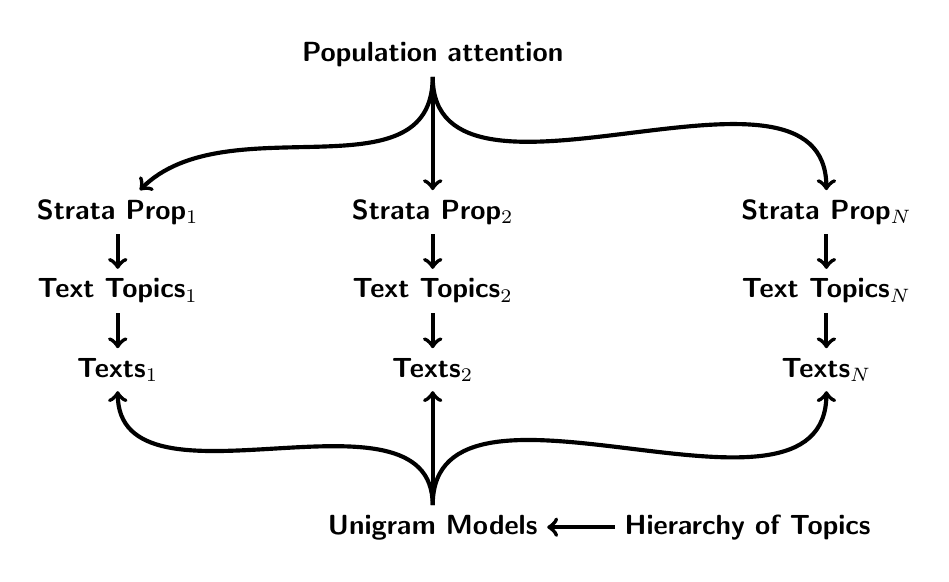
\begin{tikzpicture}

\node (col) at (-1, 10)[] {\textbf{Population attention}} ;

\invisible<1>{



\node (doc1) at (-5, 8) [] {\textbf{Strata Prop}$_{1}$} ;
\node (doc2) at (-1, 8) [] {\textbf{Strata Prop}$_{2}$} ;
\node (dots) at ( 2, 8) [] {$\hdots$} ;
\node (docN) at (4, 8) [] {\textbf{Strata Prop}$_{N}$} ;



\draw[->, line width=1.5pt] (col) to [out=270, in = 45] (doc1);
\draw[->, line width=1.5pt] (col) to [out=270, in = 90] (doc2);
\draw[->, line width=1.5pt] (col) to [out=270, in = 90] (docN);




}

\invisible<1-2>{


\node (word11) at (-5, 7) [] {\textbf{Text Topics}$_{1}$} ;
\node (word22) at (-1, 7) [] {\textbf{Text Topics}$_{2}$} ;
\node (wordnn) at (4, 7) [] {\textbf{Text Topics}$_{N}$ } ;

\draw[->, line width=1.5pt] (doc1) to [out=270, in=90] (word11) ;
\draw[->, line width=1.5pt] (doc2) to [out=270, in=90] (word22) ;
\draw[->, line width=1.5pt] (docN) to [out=270, in=90] (wordnn) ;




}



\invisible<1-3>{

\node (wordaa) at (-5, 6) [] {\textbf{Texts}$_{1}$} ;
\node (wordbb) at (-1, 6) [] {\textbf{Texts}$_{2}$} ;
\node (wordcc) at (4, 6) [] {\textbf{Texts}$_{N}$ } ;


\draw[->, line width = 1.5pt] (word11) to [out = 270, in = 90] (wordaa);
\draw[->, line width = 1.5pt] (word22) to [out = 270, in = 90] (wordbb);
\draw[->, line width = 1.5pt] (wordnn) to [out = 270, in = 90] (wordcc);

\node (topics) at (-1, 4) [] {$\textbf{Unigram Models}$} ;



\draw[->, line width = 1.5pt] (topics) to [out = 90, in = 270] (wordaa);
\draw[->, line width = 1.5pt] (topics) to [out = 90, in = 270] (wordbb);
\draw[->, line width = 1.5pt] (topics) to [out = 90, in = 270] (wordcc);



}

\invisible<1-4>{
\node (mix) at (3, 4) [] {\textbf{Hierarchy of Topics}} ;
\draw[->, line width = 1.5pt] (mix) to [out = 180, in = 0] (topics);
}


\end{tikzpicture}


\pause \pause \pause \pause \pause

\end{frame}

\begin{frame}
\frametitle{Why Encode Structure in Extensions of LDA?}

\pause

\begin{itemize}
\invisible<1>{\item[-] Substantive reasons} \pause
\begin{itemize}
\invisible<1-2>{\item[-] Additional structure corresponds to substantively interesting content} \pause
\invisible<1-3>{\item[-] Avoids potential ad-hoc secondary analysis} \pause
\invisible<1-4>{\item[-] Clear data generating process} \pause
\end{itemize}
\invisible<1-5>{\item[-] Statistical reasons} \pause
\begin{itemize}
\invisible<1-6>{\item[-] \alert{Smoothing}$\leadsto$ borrow information across groups intelligently} \pause
\invisible<1-7>{\item[-] \alert{Uncertainty}$\leadsto$ potential for better uncertainty estimates} \pause
\invisible<1-8>{\item[-] \alert{Improved topics}$\leadsto$ small word conditions, structure could help}
\end{itemize}
\end{itemize}





\end{frame}




\begin{frame}
\frametitle{Plan for the Class}

\begin{itemize}
\item[1)] Discuss model with unknown covariates for strata proportions$\leadsto$ presentational style
\item[2)] Discuss model with hierarchy of topics$\leadsto$ mirrors genre
\end{itemize}


\end{frame}



\begin{frame}
\frametitle{Unknown Covariates for Issue Attention: Measuring Attention in Senate Press Releases}

Substantive problem: \pause  \\
\invisible<1>{Senators (representatives) regularly engage the public $\rightarrow$ presentational style\\
But we know little about this engagement} \pause \\
\invisible<1-2>{Why?  \alert{Hard to Measure} } \pause \\

\invisible<1-3>{Describe model that facilitates estimation of \alert{presentational styles} in Senate press releases} \pause
\begin{itemize}
\invisible<1-4>{\item[-] Characterize representation provided to constituents} \pause
\invisible<1-5>{\item[-] Divide attention over a set of topics} \pause
\invisible<1-6>{\item[-] Given attention to topics, write press releases}
\end{itemize}
\end{frame}







\begin{frame}
\frametitle{Presentational Styles$\leadsto$ Objective Function}
\begin{itemize}
\item[-] $\pi_{itk} \equiv$ Attention senator $i$ allocates to
issue $k$ in year $t$
\item[-] $\pi_{itk} \equiv$ Probability press release is
about issue $k$
\item[-] $\boldsymbol{\pi}_{it} = (\pi_{it1},
\hdots, \pi_{it 44}) $
\end{itemize}
\pause
\invisible<1>{Press release-level parameters (press release $j$ from senator $i$
in year $t$)} \pause
\begin{itemize}
\invisible<1-2>{\item[-] \alert{Assume}: Each press release $j$
assigned to one topic.
\item[-] Let
$\boldsymbol{\tau}_{ijt}$ indicate press release $j$'s topic.} \pause
\end{itemize}
\invisible<1-3>{\begin{center} $\boldsymbol{\tau}_{ijt} \sim
\text{Multinomial}(1, \boldsymbol{\pi}_{it}) $ \end{center}} \pause
\begin{itemize}
\invisible<1-4>{\item[-] Conditional on topic, draw document's
content.} \pause
\invisible<1-5>{\item[-] If $\tau_{ijtk} =1$ then
\end{itemize}
\begin{center}$\boldsymbol{x}_{ijt} \sim \text{Multinomial}(n_{ijt}, \boldsymbol{\theta}_k
).$}
\end{center}
\end{frame}

\begin{frame}
\frametitle{Priors}

 Each $\boldsymbol{\pi}_{it}$ is a draw from one-of-$S$ styles$\leadsto$ mixture of Dirichlet distributions \pause .
\begin{eqnarray}
 \invisible<1>{\boldsymbol{\sigma}_{it} & \sim  & \text{Multinomial}(1, \boldsymbol{\beta}). } \pause \nonumber \\
 \invisible<1-2>{\boldsymbol{\pi}_{it}|\sigma_{its}=1, \boldsymbol{\alpha}_s & \sim &  \text{Dirichlet}(\boldsymbol{\alpha}_s) \nonumber } \pause \\
\invisible<1-3>{\alpha_{ks} & \sim & \text{Gamma}(0.25, 1)} \pause  \nonumber
\end{eqnarray}

\invisible<1-4>{Other priors:} \pause
\begin{eqnarray}
\invisible<1-5>{\boldsymbol{\theta}_k & \sim & \text{Multinomial}(\boldsymbol{\lambda}) \nonumber \\} \pause
\invisible<1-6>{\boldsymbol{\beta} & \sim & \text{Multinomial}(\boldsymbol{1})}
\nonumber
\end{eqnarray}

\end{frame}



%\begin{frame}
%\begin{eqnarray}
%\alpha_{sk} & \sim & \text{Gamma}(0.25, 1) \text{ for all } k, s \nonumber \\
%\boldsymbol{\beta} & \sim & \text{Dirichlet}(\boldsymbol{1}) \nonumber \\
%\boldsymbol{\theta}_k & \sim & \text{Dirichlet}(\boldsymbol{\lambda} ) \nonumber \\
%\boldsymbol{\sigma}_{it} | \boldsymbol{\beta} & \sim & \text{Multinomial}(1, \boldsymbol{\beta} ) \text{ for all } i ; t \nonumber \\
%\boldsymbol{\pi}_{it} | \boldsymbol{\sigma}_{its}=1, \boldsymbol{\alpha}_s & \sim & \text{Dirichlet}(\boldsymbol{\alpha}_s) \text{ for all } i ; t  \nonumber \\
%\boldsymbol{\tau}_{ijt}|\boldsymbol{\pi}_{it} & \sim & \text{Multinomial}(1, \boldsymbol{\pi}_{it} ) \text{ for all } j ; t ; i  \nonumber \\
%\boldsymbol{y}_{ijt} | \boldsymbol{\tau}_{ijtk} = 1,
%\boldsymbol{\theta}_k & \sim & \text{Multinomial}(n_{ijt},
%\boldsymbol{\theta}_k) \text{ for all } j ; t ; i  \nonumber
%\end{eqnarray}
%\end{frame}


\begin{frame}
\frametitle{Presentational Styles$\leadsto$ Objective Function}

\pause
\begin{eqnarray}
\invisible<1>{\boldsymbol{\beta}& \sim & \text{Dirichlet}(\boldsymbol{1}) \nonumber } \\
\invisible<1>{\boldsymbol{\theta}_{k} & \sim & \text{Dirichlet}(\boldsymbol{\lambda}) \nonumber}  \\
\invisible<1>{\alpha_{ks} & \sim & \text{Gamma}(0.25, 1) \nonumber}  \\
\invisible<1-2>{\boldsymbol{\sigma}_{it} & \sim & \text{Multinomial}(1, \boldsymbol{\beta}) \nonumber } \\
\invisible<1-3>{\boldsymbol{\pi}_{it}| \sigma_{its} = 1, \boldsymbol{\alpha}_{s} & \sim & \text{Dirichlet}(\boldsymbol{\alpha}_{s})\nonumber} \\
\invisible<1-4>{\boldsymbol{\tau}_{ijt} | \boldsymbol{\pi}_{it} & \sim & \text{Multinomial}(1, \boldsymbol{\pi}_{it}) \nonumber \\}
\invisible<1-5>{\boldsymbol{x}_{ijt}| \tau_{ijtk} = 1, \boldsymbol{\theta}_{k} & \sim & \text{Multinomial}(n_{ijt}, \boldsymbol{\theta}_{k})\nonumber }
\end{eqnarray}


\pause \pause \pause \pause \pause
\end{frame}


\begin{frame}
\frametitle{Mixture of Styles, Mixture of Topics}

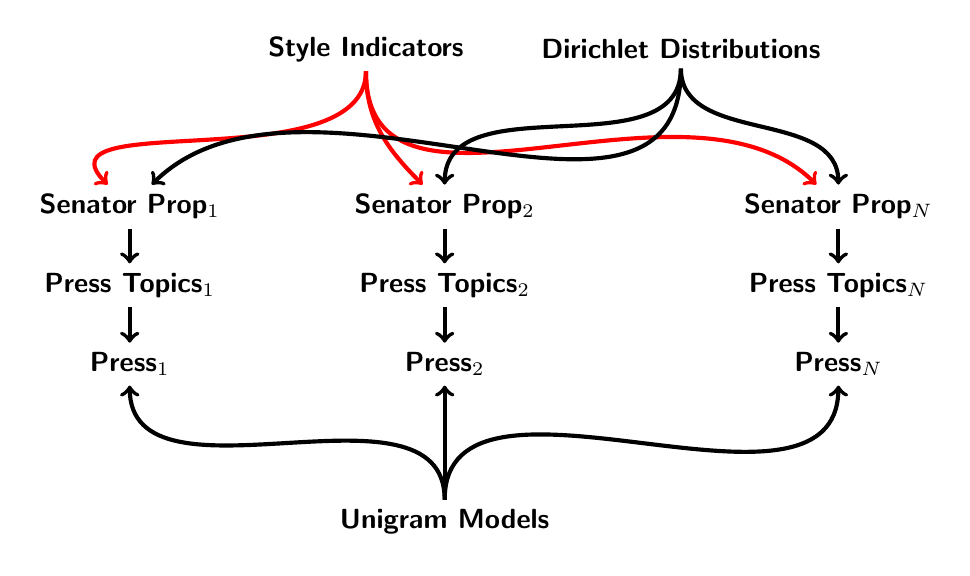
\begin{tikzpicture}

\node (col1) at (-2, 10) [] {\textbf{Style Indicators} } ;
\node (col) at (2, 10) [] {\textbf{Dirichlet Distributions} }  ;




\node (doc1) at (-5, 8) [] {\textbf{Senator Prop}$_{1}$} ;
\node (doc2) at (-1, 8) [] {\textbf{Senator Prop}$_{2}$} ;
\node (dots) at ( 2, 8) [] {$\hdots$} ;
\node (docN) at (4, 8) [] {\textbf{Senator Prop}$_{N}$} ;


\draw[->, line width=1.5pt, red] (col1) to [out=270, in = 135] (doc1);
\draw[->, line width=1.5pt, red] (col1) to [out=270, in = 135] (doc2);
\draw[->, line width=1.5pt, red] (col1) to [out=270, in = 135] (docN);



\draw[->, line width=1.5pt] (col) to [out=270, in = 45] (doc1);
\draw[->, line width=1.5pt] (col) to [out=270, in = 90] (doc2);
\draw[->, line width=1.5pt] (col) to [out=270, in = 90] (docN);





\node (word11) at (-5, 7) [] {\textbf{Press Topics}$_{1}$} ;
\node (word22) at (-1, 7) [] {\textbf{Press Topics}$_{2}$} ;
\node (wordnn) at (4, 7) [] {\textbf{Press Topics}$_{N}$ } ;

\draw[->, line width=1.5pt] (doc1) to [out=270, in=90] (word11) ;
\draw[->, line width=1.5pt] (doc2) to [out=270, in=90] (word22) ;
\draw[->, line width=1.5pt] (docN) to [out=270, in=90] (wordnn) ;



\node (wordaa) at (-5, 6) [] {\textbf{Press}$_{1}$} ;
\node (wordbb) at (-1, 6) [] {\textbf{Press}$_{2}$} ;
\node (wordcc) at (4, 6) [] {\textbf{Press}$_{N}$ } ;


\draw[->, line width = 1.5pt] (word11) to [out = 270, in = 90] (wordaa);
\draw[->, line width = 1.5pt] (word22) to [out = 270, in = 90] (wordbb);
\draw[->, line width = 1.5pt] (wordnn) to [out = 270, in = 90] (wordcc);

\node (topics) at (-1, 4) [] {$\textbf{Unigram Models}$} ;



\draw[->, line width = 1.5pt] (topics) to [out = 90, in = 270] (wordaa);
\draw[->, line width = 1.5pt] (topics) to [out = 90, in = 270] (wordbb);
\draw[->, line width = 1.5pt] (topics) to [out = 90, in = 270] (wordcc);



\end{tikzpicture}



\end{frame}



\begin{frame}

Posterior: \tiny
\begin{eqnarray}
p(\boldsymbol{\alpha}, \boldsymbol{\beta}, \boldsymbol{\theta},
\boldsymbol{\sigma}, \boldsymbol{\pi},
\boldsymbol{\tau}|\boldsymbol{X}) & \propto &
\prod_{k=1}^{K}\prod_{s=1}^{S} \frac{\exp( -
\frac{\alpha_{ks}}{1/4})}{1/4} \times \frac{\Gamma(\sum_{w=1}^{W}
\lambda_w) }{\prod_{w=1}^{W} \Gamma(\lambda_w) } \prod_{w=1}^{W}
\theta_{k,w}^{\lambda_w - 1}
\times \nonumber \\
& & \prod_{i=1}^{N} \prod_{t=2005}^{2007} \prod_{s=1}^{S} \left[
\beta_s \frac{\Gamma(\sum_{k=1}^{K} \alpha_{ks})}{\prod_{k=1}^{K}
\Gamma(\alpha_{ks} )} \prod_{k=1}^{K} \pi_{itk}^{\alpha_{ks}-1}
\prod_{j=1}^{D_{it} }\prod_{k=1}^{K} \left[ \pi_{itk}
\prod_{w=1}^{W} \theta_{kw} ^{x_{ijtw} }
 \right]^{\tau_{ijtk}} \right]^{\sigma_{its}} \nonumber
\end{eqnarray}

\pause


\normalsize
\begin{itemize}
\invisible<1>{\item[1)] Estimate with Variational Approximation} \pause
\invisible<1-2>{\item[2)] Determining number of clusters at top? (Grimmer, Shorey, Wallach, and Zlotnick, In Progress)} \pause
\begin{itemize}
\invisible<1-3>{\item[-] Non-parametric model$\leadsto$ statistical selection} \pause
\invisible<1-4>{\item[-] Experiments/Coding Exercises to assess}
\end{itemize}

\end{itemize}


\end{frame}


\begin{frame}


\only<1>{\scalebox{0.35}{\includegraphics{ShelbyPress.pdf}}}
\only<2>{\scalebox{0.35}{\includegraphics{SessionsPress.pdf}}}




\end{frame}


\begin{frame}
\frametitle{Notions of validity: From Quinn, Monroe, et al (2010) }

\begin{enumerate}
\item[-] \alert{Semantic Validity:} All categories are coherent and meaningful
\item[-] \alert{Convergent Construct Validity:} Measures concur with existing measures in critical details.
\item[-]  \alert{Discriminant Construct Validity}: Measures differ from existing measures in productive ways.
\item[-] \alert{Predictive Measure:} Measures from the model corresponds to external events in expected ways.
\item[-] \alert{Hypothesis Validity:} Measures generated from the model can be used to test substantive hypotheses.
\end{enumerate}

To establish utility of new measures, demonstrate variety of \alert{validations}\\
\alert{None of these validations are performed using a canned statistic}\\
\alert{All}: require substantive knowledge on areas (and what we expect!) [

\end{frame}


\begin{frame}
\frametitle{Home Style Measures, Semantic Validity}


\alert{Must}: Demonstrate to reader that topics are coherent and semantically meaningful

\begin{tabular}{lll}
\hline\hline
Description & Stems & \% \\
\hline
Honorary& honor,prayer,rememb,fund,tribut& 5.0\\
Transp. Grants& airport,transport,announc,urban,hud&4.8\\
Iraq& iraq,iraqi,troop,war,sectarian& 4.7\\
DHS Policy& homeland,port,terrorist,dh,fema&4.1\\
Judicial Nom.& judg,court,suprem,nomin,nomine&3.8\\
Fire Dept. Grant& firefight,homeland,afgp,award,equip&3.7\\
\hline
\end{tabular}

How: \alert{examples} in text are also useful.


\end{frame}


\begin{frame}
\frametitle{Home Style Measures, Convergent Validity}

\only<1-3>{\alert{Over time variation} }
\only<4>{\alert{Supervised/Unsupervised Convergence} }
\only<1>{\scalebox{0.4}{\includegraphics{ImmigrationPlot.pdf}}}
\only<2>{\scalebox{0.4}{\includegraphics{IraqWarPlot.pdf}}}
%\only<3>{\scalebox{0.4}{\includegraphics{Worker5.pdf}}}
\only<3>{\scalebox{0.4}{\includegraphics{HonorPlot.pdf}}}

\only<4>{\scalebox{0.3}{\includegraphics{SupervisedUnsupervised.pdf}}}
\only<5>{\scalebox{0.3}{\includegraphics{ConvValid.pdf}}}

\end{frame}


\begin{frame}
\frametitle{Discriminant Construct Validity}

\scalebox{0.45}{\includegraphics{IdealAttn.pdf} }


\end{frame}



\begin{frame}
\frametitle{Predictive Validity}


\scalebox{0.4}{\includegraphics{CompareLeaders.pdf} }


\end{frame}


\begin{frame}
\frametitle{Hypothesis Validity}


\scalebox{0.28}{\includegraphics{PrioritiesPlotLabel.pdf}}

\begin{columns}[]
\invisible<1>{\column{0.25\textwidth}
\textcolor{blue}{Senate}\\
\textcolor{blue}{Statesperson}
\begin{itemize}
\item[-] \textcolor{blue}{Iraq War}
\item[-] \textcolor{blue}{Intelligence}
\item[-] \textcolor{blue}{Intl. Relations}
\item[-] \textcolor{blue}{Budget}
\end{itemize}}

\invisible<1-2>{\column{0.25\textwidth}
\textcolor{darkgreen}{Domestic}\\
\textcolor{darkgreen}{Policy}
\begin{itemize}
\item[-] \textcolor{darkgreen}{Environment}
\item[-] \textcolor{darkgreen}{Gas prices}
\item[-] \textcolor{darkgreen}{DHS}
\item[-] \textcolor{darkgreen}{Consumer Safety}
\end{itemize}}

\invisible<1-3>{\column{0.25\textwidth} \textcolor{brown}{Pork \&
Policy}
\begin{itemize}
\item[-] \textcolor{brown}{WRDA grants}
\item[-] \textcolor{brown}{Farming}
\item[-] \textcolor{brown}{Health Care}
\item[-] \textcolor{brown}{Education Policy}
\end{itemize}}

\invisible<1-4>{\column{0.25\textwidth}
\textcolor{red}{Appropriators}
\begin{itemize}
\item[-] \textcolor{red}{Fire Grants}
\item[-] \textcolor{red}{Airport Grants}
\item[-] \textcolor{red}{University Money}
\item[-] \textcolor{red}{Police Grants}
\end{itemize}}


\end{columns}

\pause\pause\pause\pause
\end{frame}

\begin{frame}
\frametitle{Hypothesis Validity}


Why do senators adopt different styles?\\
\alert{District Fit}

\scalebox{0.4}{\includegraphics{FinalAvoidance.pdf}}



\end{frame}


\begin{frame}
\frametitle{What are the right number of topics?}

\pause

\begin{itemize}
\invisible<1>{\item[-] Number of topics$\leadsto$ depends on task at hand}
\invisible<1-2>{\item[-] Coarse$\leadsto$ broad comparisons, lose distinctions}
\invisible<1-3>{\item[-] Granular$\leadsto$ specific insights, lose broader picture}
\invisible<1-4>{\item[-] \alert{Hierarchy of topics}$\leadsto$ Pachinko Allocation, Hierarchies of von-Mises Fisher Distributions}
\end{itemize}

\invisible<1-5>{Blaydes, Grimmer, and McQueen 2017$\leadsto$ estimate nested topics to explore the \alert{Mirros for Princes}}


\pause \pause \pause \pause



\end{frame}




\begin{frame}
\frametitle{The Mirrors Genre (BGM 2017)}


26 Christian mirrors \pause
\begin{itemize}
\invisible<1>{\item[-] The Prince (1513 CE)} \pause
\invisible<1-2>{\item[-] Advice to Justinian (527 CE)} \pause
\invisible<1-3>{\item[-] The Adventures of Telemachus (1699 CE)} \pause
\end{itemize}


\invisible<1-4>{21 Islamic texts} \pause
\begin{itemize}
\invisible<1-5>{\item[-] Advice on the Art of Governance (1612 CE)} \pause
\invisible<1-6>{\item[-] Kalila wa Dimna (748 CE)} \pause
\invisible<1-7>{\item[-] The Sultan's Register of Laws (1632-1633 CE)} \pause
\end{itemize}



\invisible<1-8>{Work with translations}\pause\invisible<1-9>{$\leadsto$ little evidence of selection} \pause
\begin{itemize}
\invisible<1-10>{\item[-] Collect data on collection of 98 (51 Christian, 47 Islamic, some not translated)} \pause
\invisible<1-11>{\item[-] No difference on Year/Region}
\end{itemize}


\end{frame}




\begin{frame}
\frametitle{Preprocessing Texts}

47 books \invisible<1>{$\leadsto$ Each divided into paragraphs} \\
\invisible<1-2>{Create feature space}
\begin{itemize}
\invisible<1-3>{\item[-] Bag of words, stem, discard punctuation, stop words}
\invisible<1-4>{\item[-] Translate words left in Arabic (\alert{allah}) and discard proper nouns}
\invisible<1-5>{\item[-] Identified synonyms}
\begin{itemize}
\invisible<1-6>{\item[-] \alert{almighty}, \alert{god}}
\invisible<1-7>{\item[-] \alert{monarch}, \alert{prince}, \alert{king}, \alert{ruler}}
\invisible<1-8>{\item[-] \alert{Lord} $\neq$ \alert{lord} }
\end{itemize}
\end{itemize}

\invisible<1-9>{Result: short segment $j$ in book $i$ is a count vector}
\begin{eqnarray}
\invisible<1-10>{\textbf{x}_{ij} & = & (x_{ij1}, x_{ij2}, \hdots, x_{ij2124}) \nonumber}
\end{eqnarray}

\invisible<1-11>{We work with a normalized version of the documents, }
\begin{eqnarray}
\invisible<1-12>{\textbf{x}^{*}_{ij} & = & \frac{\textbf{x}_{ij}}{\sqrt{\textbf{x}^{'}_{ij}\textbf{x}_{ij}} } \nonumber}
\end{eqnarray}



\pause \pause \pause \pause \pause \pause \pause \pause \pause \pause \pause \pause


\end{frame}




\begin{frame}
\frametitle{Measuring Themes in the Mirrors}

\only<1-3>{Model built around two hierarchies:
\begin{itemize}
\invisible<1>{\item[1)] Books $\leadsto$ paragraphs (Blei, Ng, Jordan 2003; Wallach, 2008; Quinn et al 2010; Grimmer 2010; Roberts et al 2014)}
\invisible<1-2>{\item[2)] Coarse topics $\leadsto$ granular topics (Li and McCallum 2006; Gopal and Yang 2014)}
\end{itemize}
}


\only<4->{
Estimate \alert{four} quantities of interest
\begin{itemize}
\invisible<1-4>{\item[1)] Granular topics (60)}
\invisible<1-5>{\item[2)] Coarse (broad) topics (3)}
\begin{itemize}
\invisible<1-6>{\item[-] Each granular topic classified into one coarse topic }
\end{itemize}
\invisible<1-7>{\item[3)] Each book $i'$s  $\textbf{themes}_{i}}$
\invisible<1-8>{\item[4)] Each short segment's granular (and coarse) topic }
\end{itemize}




\begin{eqnarray}
\invisible<1-7, 9->{\textbf{themes}_{i} & = & (\text{theme}_{i1}, \text{theme}_{i2}, \hdots, \text{theme}_{i60} ) \nonumber }
\end{eqnarray}

}



\pause \pause \pause \pause \pause \pause \pause \pause
\end{frame}

\begin{frame}
\frametitle{A Hierarchy of Topics}


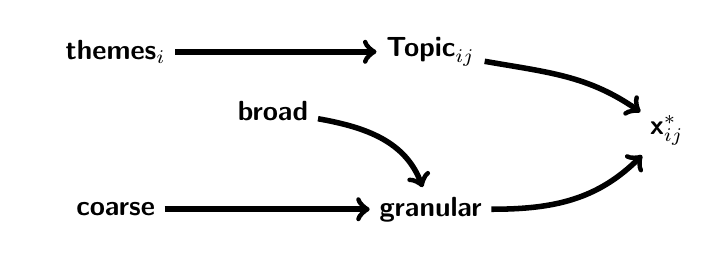
\begin{tikzpicture}

\node (Dummy) at (-9,8) [] {} ;
\node (theme1) at (-8, 9) [] {$\textbf{themes}_{i} $} ;
\invisible<1>{\node (draws) at (-4, 9) [] {$\textbf{Topic}_{ij}$};}
\invisible<1>{\draw[->, line width = 2pt] (theme1) to [out = 0, in = 180] (draws);}

\invisible<1-2>{\node (document) at (-1, 8) [] {$\textbf{x}^{*}_{ij}$ }; }
\invisible<1-2>{\draw[->, line width = 2pt] (draws) to [out = 350, in  = 145] (document); }


\invisible<1-2>{\node (topics)   at (-4, 7) [] {$\textbf{granular}$}; }

\invisible<1-2>{\draw[->, line width = 2pt] (topics) to [out = 0, in = 225] (document) ; }

\invisible<1-3>{\node (topic_sig) at (-6, 8.25) [] {$\textbf{broad}$} ; }

\invisible<1-3>{\draw[->, line width = 2pt] (topic_sig) to [out = 350, in = 110] (topics) ; }

\invisible<1-3>{\node (coarse)    at (-8, 7) [] {$\textbf{coarse}$}; }

\invisible<1-3>{\draw[->, line width = 2pt] (coarse) to [out = 0, in= 180] (topics) ; }

\end{tikzpicture}


\begin{eqnarray}
\invisible<1>{\textbf{Topic}_{ij} & \sim & \text{Multinomial}(1, \textbf{themes}_{i}) \nonumber }\\
\invisible<1-2>{\textbf{x}^{*}_{ij} | \text{Topic}_{ijk} =  1 & \sim & \text{vMF} (\kappa, \textbf{granular}_{k} ) \nonumber }\\
\invisible<1-3>{\textbf{broad}_{k} & \sim & \text{Multinomial}(1, \textbf{Broad Theme Prior}) \nonumber }\\
\invisible<1-3>{\textbf{granular}_{k} | \text{broad}_{km} = 1 & \sim & \text{vMF}(\kappa, \textbf{coarse}_{m}) \nonumber }
\end{eqnarray}

\invisible<1-4>{Estimate model with Variational Approximation}\\
\invisible<1-5>{Model selection: automatic model fit, qualitative evaluation}

\pause \pause \pause \pause \pause




%%draws theme
%%then draws content from a topic specific distribution
%%our model classifies each of those granular themes into coarse themes



\end{frame}





\begin{frame}
\frametitle{Interpreting Unsupervised Models}

Two approaches to labeling output \pause
\begin{itemize}
\invisible<1>{\item[1)] \alert{Computational}: identify discriminating words }\pause
\invisible<1-2>{\item[2)] \alert{Manual}: Segments classified to coarse, granular topics.  Read, discuss, and label} \pause
\end{itemize}

\invisible<1-3>{Unsupervised models \alert{structure} and \alert{guide} our reading}




\end{frame}



\begin{frame}
\frametitle{Art of Rulership}


Practices and ideals of political rule

\vspace{0.5in}
\begin{tabular}{l}
\invisible<1>{king}\invisible<1-2>{,princ}\invisible<1-3>{,citi}\invisible<1-4>{,great,place,work,emperor,enemi,armi,letter} \\
\end{tabular}

\vspace{0.5in}
 \invisible<1-5>{36.5\% of paragraphs }

\pause \pause \pause \pause \pause


\end{frame}

\begin{frame}

\begin{center}
\scalebox{0.45}{\includegraphics{Hist_Super1_p.pdf}}
\end{center}

\end{frame}


\begin{frame}

\begin{center}
\scalebox{0.45}{\includegraphics{Super1.pdf}}
\end{center}


\end{frame}


\begin{frame}
\frametitle{Religion and Virtue}


Connection between religion, virtue, justice and political rule \pause

\vspace{0.5in}
\begin{tabular}{l}
\invisible<1>{almighti,good,virtu,power,ruler,justic,prayer,rule,prophet,mena \\}
\end{tabular}

\pause
\vspace{0.5in}

\invisible<1-2>{32.2\% of pargraphs}

\end{frame}


\begin{frame}

\begin{center}
\scalebox{0.45}{\includegraphics{Hist_Super2_p.pdf}}
\end{center}

\end{frame}



\begin{frame}

\begin{center}
\scalebox{0.45}{\includegraphics{Super2.pdf}}
\end{center}

\end{frame}






\begin{frame}
\frametitle{Inner Life of the Ruler}

Personal relationships, care for and practices of the self, and ultimate fate of the soul \pause

\vspace{0.5in}

\begin{tabular}{ll}
\invisible<1>{man,land,woman,know,bodi,eye,ladi,love,faculti,old} \pause
\end{tabular}

\vspace{0.5in}

\invisible<1-2>{31.2\% of paragraphs}

\end{frame}



\begin{frame}


\begin{center}
\scalebox{0.45}{\includegraphics{Hist_Super3_p.pdf}}
\end{center}

\end{frame}




\begin{frame}

\begin{center}
\scalebox{0.45}{\includegraphics{Super3.pdf}}
\end{center}

\end{frame}



\begin{frame}
\frametitle{Granular: Best Practices for Ruling}


\begin{tabular}{l}
\hline
king,princ,citi,great,place,work,emperor,enemi,armi,letter \\
\hline
\alert{king,kingdom,royal,minist,reign,father,court,majesti,presenc,war}
\end{tabular}

\vspace{0.5in}

6.2\% of paragraphs

\end{frame}



\begin{frame}

\begin{center}
\scalebox{0.45}{\includegraphics{1point1.pdf}}
\end{center}

\end{frame}


\begin{frame}
\frametitle{Granular: Characteristics that distinguish Just Ruler from Tyrant}


\begin{tabular}{l}
\hline
king,princ,citi,great,place,work,emperor,enemi,armi,letter \\
\hline
king,kingdom,royal,minist,reign,father,court,majesti,presenc,war\\
\alert{princ,good,peopl,christian,tyranni,war,mind,ought,state,public}\\
\end{tabular}

\vspace{0.5in}

3.1\% of paragraphs

\end{frame}


\begin{frame}

\begin{center}
\scalebox{0.45}{\includegraphics{1point2.pdf}}
\end{center}

\end{frame}


\begin{frame}
\frametitle{Granular: Religious Virtues and Political Ideals}


\begin{tabular}{l}
\hline
almighti,good,virtu,power,ruler,justic,prayer,rule,prophet,mena\\
\hline
\alert{almighti,bless,grant,peac,messeng,prophet,merci,holi,command,grace}
\end{tabular}

\vspace{0.5in}

6.9\% of paragraphs


\end{frame}



\begin{frame}

\begin{center}
\scalebox{0.45}{\includegraphics{2point1.pdf}}
\end{center}

\end{frame}


\begin{frame}

\huge

Principal Component Analysis

\end{frame}



\begin{frame}
\frametitle{A Simple Two-Dimensional Example}

Suppose we have the following observations:
\begin{eqnarray}
x_{1} & = & (0.54, 1.07) \nonumber \\
x_{2} & = & (-1.20, -0.76) \nonumber \\
x_{3} & = & (-0.63, -0.81)\nonumber \\
x_{4} & = & (0.96, 0.75) \nonumber \\
x_{5} & = & (1.64, 1.37) \nonumber
\end{eqnarray}


\end{frame}



\begin{frame}
\begin{center}
\only<1>{\scalebox{0.6}{\includegraphics{Plot1.pdf}}}
\only<2>{
  Goal: find line that summarizes bivariate information
\scalebox{0.5}{\includegraphics{Plot1.pdf}}
}


\end{center}
\end{frame}

\begin{frame}
\frametitle{Vectors to Draw a Line}

Suppose $\boldsymbol{w}_{1} = (1,1)$
\only<1-4>{\invisible<1-3>{$2 \boldsymbol{w}_{1} = (2, 2)$ }}
\only<5>{$\frac{1}{2} \boldsymbol{w}_{1} = (1/2, 1/2)$}
\only<6>{$-2 \boldsymbol{w}_{1} = (-2, -2)$ }
\only<7>{$-\frac{1}{2} \boldsymbol{w}_{1} = (-1/2, -1/2)$ }



\begin{center}
\only<1>{\scalebox{0.5}{\includegraphics{Plot2.pdf}}}
\only<2>{\scalebox{0.5}{\includegraphics{Plot3.pdf}}}
\only<3>{\scalebox{0.5}{\includegraphics{Plot4.pdf}}}
\only<4>{\scalebox{0.5}{\includegraphics{Plot5.pdf}}}
\only<5>{\scalebox{0.5}{\includegraphics{Plot6.pdf}}}
\only<6>{\scalebox{0.5}{\includegraphics{Plot7.pdf}}}
\only<7>{\scalebox{0.5}{\includegraphics{Plot8.pdf}}}
\only<8>{
$z_{i} = $ amount we shrink/flip $\boldsymbol{w}_{1}$ to approximate point $i$.

\scalebox{0.3}{\includegraphics{Plot8.pdf}}}
\end{center}




\end{frame}



\begin{frame}

$\boldsymbol{w}_{1} = (0.75, 0.66)$
\invisible<1>{$z_{1} = 1.12$}

\begin{center}
\only<1>{\scalebox{0.5}{\includegraphics{Plot9.pdf}}}
\only<2>{\scalebox{0.5}{\includegraphics{Plot10.pdf}}}
\only<3>{\scalebox{0.5}{\includegraphics{Plot11.pdf}}}
\only<4>{\scalebox{0.5}{\includegraphics{Plot12.pdf}}}

\end{center}




\end{frame}



\begin{frame}
\frametitle{Algebraic Representation}

\begin{eqnarray}
\boldsymbol{x}_{i} & = & z_{i} \boldsymbol{w}_{1}  + \boldsymbol{e}_{i} \nonumber \pause  \\
\invisible<1>{(x_{i1}, x_{i2}) & = & (z_{i}w_{11} + e_{i1} , z_{i} w_{12} + e_{i2} )\nonumber} \pause
\end{eqnarray}

\invisible<1-2>{Find $\boldsymbol{w}_{1} = (w_{11}, w_{12}) $ and $z_{i}$ to minimize the error} \pause


\begin{eqnarray}
\invisible<1-3>{\text{error} & = & \frac{1}{N} \sum_{i=1}^{N} ((x_{i1}, x_{i2})  - z_{i}(w_{11}, w_{12}) )^{'} ((x_{i1}, x_{i2})  - z_{i}(w_{11}, w_{12}) ) \nonumber \\} \pause
\invisible<1-4>{& = & \frac{1}{N} \sum_{i=1}^{N} (x_{i1} - z_{i} w_{11} )^{2} + (x_{i2} - z_{i} w_{12} )^{2} \nonumber }
\end{eqnarray}


\end{frame}


\begin{frame}
\frametitle{Three Dimensional Approximation}

\begin{eqnarray}
\boldsymbol{x}_{1} & = & (0.09, -1.02, -0.10) \nonumber \\
\boldsymbol{x}_{2} & = & (0.09, 1.41, 0.67) \nonumber \\
\boldsymbol{x}_{3} & = & (-0.81, -1.46, -0.54) \nonumber \\
\boldsymbol{x}_{4} & = & (1.43, 0.26, 0.61)\nonumber \\
\boldsymbol{x}_{5} & = & (1.23, 0.87, 1.33\nonumber
\end{eqnarray}

Find $\boldsymbol{w}_{1} = (w_{11}, w_{12}, w_{13})$ and $z_{i}$ to provide best one dimensional approximation.


\end{frame}


\begin{frame}

{\tt Three-Dimensional Visualization}

\only<2>{$\boldsymbol{w}_{1} = (0.48, 0.75, 0.46)$}


\end{frame}



\begin{frame}
\begin{eqnarray}
\boldsymbol{x}_{i} & = & z_{i} \boldsymbol{w}_{1}  + \boldsymbol{e}_{i} \nonumber \pause  \\
\invisible<1>{(x_{i1}, x_{i2}, x_{i3}) & = & (z_{i}w_{11} + e_{i1} , z_{i} w_{12} + e_{i2}, z_{i} w_{13} + e_{i3} )\nonumber} \pause
\end{eqnarray}

\invisible<1-2>{Find $\boldsymbol{w}_{1} = (w_{11}, w_{12}, w_{13}) $ and $z_{i}$ to minimize the error} \pause


\begin{eqnarray}
\invisible<1-3>{\text{error} & = & \frac{1}{N} \sum_{i=1}^{N} ((x_{i1}, x_{i2}, x_{13})- z_{i}(w_{11}, w_{12}, w_{13}) )^{'} \nonumber \\
&&   ((x_{i1}, x_{i2}, x_{i3})  - z_{i}(w_{11}, w_{12}, w_{13}) ) \nonumber} \pause  \\
\invisible<1-4>{& = & \frac{1}{N} \sum_{i=1}^{N} (x_{i1} - z_{i} w_{11} )^{2} + (x_{i2} - z_{i} w_{12} )^{2} + (x_{i3} - z_{i} w_{13} )^{2}  \nonumber}
\end{eqnarray}



\end{frame}



\begin{frame}
\frametitle{Principal Component Analysis}

\only<1>{\scalebox{0.5}{\includegraphics{PrCompExamp1.pdf}}}
\only<2>{\scalebox{0.5}{\includegraphics{PrCompExamp2.pdf}}}
\only<3>{\scalebox{0.5}{\includegraphics{PrCompExamp3.pdf}}}



\end{frame}



\begin{frame}
\frametitle{PCA Output}
$\boldsymbol{x}_{i} = (x_{i1}, x_{i2}, \hdots, x_{iJ})$ \pause



\invisible<1>{Principal Component Output:} \pause

\begin{itemize}
\invisible<1-2>{\item[1)] $K$ Principal Components $\boldsymbol{w}_{k}$ } \pause
\begin{eqnarray}
\invisible<1-3>{\boldsymbol{w}_{k} & = & (w_{1k}, w_{2k}, \hdots, w_{Jk})\nonumber } \pause
\end{eqnarray}
\invisible<1-4>{\item[2)] $K$ component vector describing loadings on principal components for each document } \pause
\begin{eqnarray}
\invisible<1-5>{\boldsymbol{z}_{i} & = & (z_{1i}, z_{2i}, \hdots, z_{Ki}) \nonumber }
\end{eqnarray}
\end{itemize}


\end{frame}




\begin{frame}
\frametitle{An Introduction to Eigenvectors, Values, and Diagonalization}


\begin{defn}
Suppose $\boldsymbol{A}$ is an $N \times N$ matrix and $\lambda$ is a scalar.  \\

If

\begin{eqnarray}
\boldsymbol{A}\boldsymbol{x} &= & \lambda \boldsymbol{x} \nonumber
\end{eqnarray}

Then $\boldsymbol{x}$ is an \alert{eigenvector} and $\lambda$ is the associated \alert{eigenvalue}


\end{defn}

\pause

\begin{itemize}
\invisible<1>{\item[-] $\boldsymbol{A}$ stretches the eigenvector $\boldsymbol{x}$ } \pause
\invisible<1-2>{\item[-] $\boldsymbol{A}$ stretches $\boldsymbol{x}$ by $\lambda$ } \pause
\invisible<1-3>{\item[-] To find eigenvectors/values: ({\tt eigen} in {\tt R} ) } \pause
\begin{itemize}
\invisible<1-4>{\item Find $\lambda$ that solves $\text{det}(\boldsymbol{A}- \lambda \boldsymbol{I}) = 0 $} \pause
\invisible<1-5>{\item Find vectors in \alert{null space} of:} \pause
\begin{eqnarray}
\invisible<1-6>{(\boldsymbol{A} - \lambda \boldsymbol{I} ) &= & 0 \nonumber }
\end{eqnarray}
\end{itemize}
\end{itemize}


\end{frame}




\begin{frame}
\frametitle{Finding a Lower Dimensional Space (Manifold Learning)}
\begin{center}
\only<1>{\scalebox{0.5}{\includegraphics{PrCompExamp1.pdf}}}
\only<2>{\scalebox{0.5}{\includegraphics{PrCompExamp2.pdf}}}
\only<3>{\scalebox{0.5}{\includegraphics{PrCompExamp3.pdf}}}
\end{center}
\only<4-7>{
\begin{center}
\scalebox{0.15}{\includegraphics{PrCompExamp3.pdf}}
\end{center}
Original data:
\begin{eqnarray}
\invisible<1-4>{\boldsymbol{x}_{i} & = &  (x_{i1}, x_{i2}) \nonumber }
\end{eqnarray}

\invisible<1-5>{Which we approximate with }
\begin{eqnarray}
\invisible<1-6>{\tilde{\boldsymbol{x}}_{i} & = & z_{i} \boldsymbol{w}_{1} \nonumber \\
& =& z_{i} (w_{11}, w_{12}) \nonumber }
\end{eqnarray}
}

\only<8->{
\begin{center}
\scalebox{0.15}{\includegraphics{PrCompExamp3.pdf}}
\end{center}

Original data $\boldsymbol{x}_{i} \in \Re^{J}$
\begin{eqnarray}
\boldsymbol{x}_{i} & = & (x_{i1}, x_{i2}, \hdots, x_{iJ}) \nonumber
\end{eqnarray}

Which we approximate with $L\leq J$ weights $z_{il}$ and vectors $\boldsymbol{w}_{l} \in \Re^{J}$
\begin{eqnarray}
\tilde{\boldsymbol{x}}_{i} & = & z_{i1} \boldsymbol{w}_{1} + z_{i2} \boldsymbol{w}_{2} + \hdots + z_{iL} \boldsymbol{w}_{L} \nonumber
\end{eqnarray}

Define $\boldsymbol{\theta} = (\underbrace{\boldsymbol{Z}}_{N \times L}, \underbrace{\boldsymbol{W}_{L}}_{L \times J} )$

}
\pause \pause \pause \pause \pause \pause




\end{frame}







\begin{frame}
\frametitle{Principal Component Analysis$\leadsto$ Objective function}

Consider 1-dimensional case ($L = 1$), centered data, and $||\boldsymbol{w}_{1}|| = 1$.  \pause  \\
\begin{eqnarray}
\invisible<1>{f(\boldsymbol{\theta},  \boldsymbol{X}) & = & \frac{1}{N} \sum_{i=1}^{N} ||\boldsymbol{x}_{i} - z_{i1}\boldsymbol{w}_{1} ||^2  } \pause  \nonumber \\
\invisible<1-2>{& = & \frac{1}{N} \sum_{i=1}^{N} (\boldsymbol{x}_{i}  - z_{i1} \boldsymbol{w}_{1} )^{'}(\boldsymbol{x}_{i}  - z_{i1} \boldsymbol{w}_{1} ) \nonumber } \pause \\
\invisible<1-3>{& = & \frac{1}{N}\sum_{i=1}^{N}\left(\boldsymbol{x}_{i}^{'}\boldsymbol{x}_{i} - 2 z_{i1}\boldsymbol{w}_{1}^{'}\boldsymbol{x}_{i} + z_{i1}^{2} \right ) \nonumber } \pause
\end{eqnarray}

\invisible<1-4>{$\boldsymbol{w}_{1}^{'}\boldsymbol{w}_{1} = 1$}
\end{frame}

\begin{frame}
\frametitle{Principal Component Analysis$\leadsto$ Optimization}


Optimization: \pause
\begin{eqnarray}
\invisible<1>{\frac{\partial f(\boldsymbol{\theta}, \boldsymbol{X})}{\partial z_{i1}}  & = &  - \frac{2 \boldsymbol{w}_{1}^{'} \boldsymbol{x}_{i} + 2 z_{i1}}{N} \nonumber \\} \pause
\invisible<1-2>{0 & = & - \frac{2 \boldsymbol{w}_{1}^{'} \boldsymbol{x}_{i} + 2 z_{i1}^{*}}{N} \nonumber \\} \pause
\invisible<1-3>{z_{i1}^{*} & = & \boldsymbol{w}_{1}^{'} \boldsymbol{x}_{i} \nonumber }
\end{eqnarray}



\end{frame}





\begin{frame}
\frametitle{Principal Component Analysis$\leadsto$ Optimization}
Substituting in $z_{i1}^{*}$ \pause

\begin{eqnarray}
\invisible<1>{& = & \frac{1}{N} \sum_{i=1}^{N} (\boldsymbol{x}_{i}  - z_{i1}^{*} \boldsymbol{w}_{1} )^{'}(\boldsymbol{x}_{i}  - z_{i1}^{*} \boldsymbol{w}_{1} ) \nonumber } \pause \\
 \invisible<1-2>{& = & \frac{1}{N} \sum_{i=1}^{N} (\underbrace{\boldsymbol{x}_{i}^{'}\boldsymbol{x}_{i}}_{\text{Constant}}  - 2 z_{i1}^{*} \underbrace{\boldsymbol{w}_{1}^{'}\boldsymbol{x}_{i}}_{z_{i1}^{*}}  + \left(z_{i1}^{*}\right)^{2} \underbrace{\boldsymbol{w}_{1}^{'}\boldsymbol{w}_{1}}_{1} )   \nonumber } \pause \\
 \invisible<1-3>{& = &  - \frac{1}{N} \sum_{i=1}^{N}   \left(z_{i1}^{*}\right)^{2} + c \nonumber } \pause \\
 \invisible<1-4>{& = & - \frac{1}{N} \sum_{i=1}^{N} \boldsymbol{w}_{1}^{'}\boldsymbol{x}_{i}\boldsymbol{x}^{'}_{i}\boldsymbol{w}_{1} \nonumber } \pause \\
 \invisible<1-5>{& = & -  \boldsymbol{w}_{1}^{'}\boldsymbol{\Sigma} \boldsymbol{w}_{1} \nonumber}
\end{eqnarray}



\end{frame}

\begin{frame}
\frametitle{Principal Component Analysis$\leadsto$ Optimization}

\begin{eqnarray}
 & = & -   \boldsymbol{w}_{1}^{'}\boldsymbol{\Sigma} \boldsymbol{w}_{1} \nonumber \pause
\end{eqnarray}


\invisible<1>{where $\boldsymbol{\Sigma}$ is the :} \pause
\begin{itemize}
\invisible<1-2>{\item[-] Empirical covariance matrix$\leadsto \frac{1}{N} \boldsymbol{X}^{'}\boldsymbol{X}$} \pause
\invisible<1-3>{\item[-] \alert{Variance} of the projected data.  Define } \pause
\begin{eqnarray}
\invisible<1-4>{\boldsymbol{z}_{1} & = & (\boldsymbol{w}_{1} \boldsymbol{x}_{1}, \boldsymbol{w}_{1} \boldsymbol{x}_{2}, \hdots, \boldsymbol{w}_{1}\boldsymbol{x}_{N}) \nonumber \\} \pause
\invisible<1-5>{\text{var}(\boldsymbol{z}_{1}) & = & E[\boldsymbol{z}_{1}^{2} ]  - E[\boldsymbol{z}_{1}]^{2} \nonumber \\} \pause
\invisible<1-6>{& = & \frac{1}{N} \sum_{i=1}^{N} z_{i1}^{2} - 0 \nonumber \\} \pause
\invisible<1-7>{& = & \frac{1}{N} \sum_{i=1}^{N} \boldsymbol{w}_{1}^{'}\boldsymbol{x}_{i}\boldsymbol{x}_{i}^{'}\boldsymbol{w}_{1}  = \boldsymbol{w}_{1}^{'} \boldsymbol{\Sigma} \boldsymbol{w}_{1} \nonumber } \pause
\end{eqnarray}

\end{itemize}

\invisible<1-8>{Minimize reconstruction error }\pause \invisible<1-9>{$\leadsto$ maximize variance of projected data}

\end{frame}


\begin{frame}
\frametitle{Principal Component Analysis$\leadsto$ Optimization}

Maximize variance, subject to constraints \pause


\begin{eqnarray}
\invisible<1>{g(\boldsymbol{z}^{*}, \boldsymbol{w}_{1}, \boldsymbol{X}) & = & \boldsymbol{w}_{1}^{'} \boldsymbol{\Sigma}\boldsymbol{w}_{1} - \lambda_{1}(\boldsymbol{w}_{1}^{'} \boldsymbol{w}_{1} - 1 ) \nonumber \\} \pause
 \invisible<1-2>{\frac{\partial g(\boldsymbol{z}^{*}, \boldsymbol{w}_{1}, \boldsymbol{X})}{\partial \boldsymbol{w}_{1}} &= & 2 \boldsymbol{\Sigma}\boldsymbol{w}_{1}  - 2 \lambda_{1} \boldsymbol{w}_{1} \nonumber \\}\pause
 \invisible<1-3>{\boldsymbol{\Sigma}\boldsymbol{w}_{1}^{*} & = &  \lambda_{1} \boldsymbol{w}_{1}^{*} \nonumber } \pause
\end{eqnarray}

\invisible<1-4>{$\alert{\boldsymbol{w}_{1}^{*}}$ = \alert{Eigenvector of $\boldsymbol{\Sigma}$}}\pause \invisible<1-5>{ (!!!!!!)} \pause \\
\invisible<1-6>{
We want $\boldsymbol{w}_{1}$ to maximize variance and } \pause
\invisible<1-7>{
  \begin{eqnarray}
\boldsymbol{w}_{1}^{'} \boldsymbol{\Sigma} \boldsymbol{w}_{1} = \lambda_{1} \nonumber
  \end{eqnarray}}\pause
\invisible<1-8>{
So $\boldsymbol{w}_{1}$ is eigenvector associated with the largest eigenvalue $\lambda_{1}$
}






\end{frame}




\begin{frame}
\frametitle{An Introduction to Eigenvectors, Values, and Diagonalization}


\begin{thm}
Suppose $\boldsymbol{A}$ is an \alert{invertible} $N \times N$ matrix with $N$ linearly independent eigenvectors.  Then we can write $\boldsymbol{A}$ as,

\begin{eqnarray}
\boldsymbol{A} &= & \boldsymbol{W}^{'}\begin{pmatrix}
\lambda_{1} & 0 & \hdots & 0 \\
0 & \lambda_{2} & \hdots & 0 \\
\vdots & \vdots & \ddots & \vdots \\
0 & 0&  \hdots & \lambda_{N}\\
\end{pmatrix}
\boldsymbol{W} \nonumber
\end{eqnarray}

where $\boldsymbol{W} = \left(\boldsymbol{w}_{1}, \boldsymbol{w}_{2}, \hdots, \boldsymbol{w}_{N} \right)$ is an $N \times N$ matrix with the $N$ eigenvectors as column vectors.

\end{thm}

\end{frame}


\begin{frame}
\frametitle{An Introduction to Eigenvectors, Values, and Diagonalization}


\begin{defn}
Suppose $A$ is a covariance matrix.  Then, we can write $A$ as

\begin{eqnarray}
\boldsymbol{A} &= & \boldsymbol{W}^{'}\begin{pmatrix}
\lambda_{1} & 0 & \hdots & 0 \\
0 & \lambda_{2} & \hdots & 0 \\
\vdots & \vdots & \ddots & \vdots \\
0 & 0&  \hdots & \lambda_{N}\\
\end{pmatrix}
\boldsymbol{W} \nonumber
\end{eqnarray}

Where $\lambda_{1}>\lambda_{2} > \hdots > \lambda_{N} \geq 0$. \\
We will call $\boldsymbol{w}_{1}$ the first eigenvector, $\boldsymbol{w}_{2}$ the second eigenvector, ..., $\boldsymbol{w}_{j}$ the $\text{j}^{th}$ eigenvector.

\end{defn}

\end{frame}


\begin{frame}
\frametitle{Back to Principal Components}


\begin{thm}
Suppose we want to approximate $N$ observations $\boldsymbol{x}_{i} \in \Re^{J}$ with $L < J$ orthogonal-unit length vectors $\boldsymbol{w}_{l} \in \Re^{J}$ with associated scores $z_{il}$ to minimize reconstruction error: \pause

\begin{eqnarray}
\invisible<1>{f(\boldsymbol{X}, \boldsymbol{\theta}) & = & \frac{1}{N} \sum_{i=1}^{N} || \boldsymbol{x}_{i}  - \sum_{l = 1}^{L} z_{il} \boldsymbol{w}_{l}||^{2} \nonumber  } \pause
\end{eqnarray}

\invisible<1-2>{The optimal solution sets each $\boldsymbol{w}_{l}$ to be the $l^{\text{th}}$ eigenvector of the empirical covariance matrix.}\pause \invisible<1-3>{Further $z_{il}^{*} = \boldsymbol{w}_{l}^{'}\boldsymbol{x}_{i}$ so that the $L$ dimensional representation is:} \pause
\begin{eqnarray}
\invisible<1-4>{\boldsymbol{x}^{L}_{i} & = & (\boldsymbol{w}_{1}^{'}\boldsymbol{x}_{i}, \boldsymbol{w}_{2}^{'}\boldsymbol{x}_{i}, \hdots, \boldsymbol{w}_{L}^{'}\boldsymbol{x}_{i} ) \nonumber }
\end{eqnarray}

\end{thm}

\end{frame}



\begin{frame}
\frametitle{Application of Principal Components in {\tt R}}

Consider press releases from 2005 US Senators \pause \\
\invisible<1>{Define $\boldsymbol{x}_{i} = (x_{i1}, x_{i2}, \hdots, x_{iJ})$ as the rate senator $i$ uses $J$ words.  }\pause
\begin{eqnarray}
\invisible<1-2>{x_{ij} & = & \frac{\text{No. Times $i$ uses word $j$}}{\text{No. words $i$ uses}} \nonumber } \pause
\end{eqnarray}

\invisible<1-3>{{\tt  dtm}: $100 \times 2796$ matrix containing word rates for senators\\} \pause
\invisible<1-4>{{\tt prcomp(dtm) } applies principal components}


\end{frame}


\begin{frame}

\begin{semiverbatim}

load("SenateTDM.RData")

dtm<- t(tdm)

for(z in 1:100)\{

  dtm[z,]<- dtm[z,]/sum(dtm[z,])

  \}


store<- prcomp(dtm, \alert{scale = F})

scores<- store\$x[,1]

\end{semiverbatim}
\end{frame}


\begin{frame}
\frametitle{Application of Principal Components in {\tt R}}


\only<1>{\scalebox{0.5}{\includegraphics{FirstPrinComp.pdf}}}
\only<2>{\scalebox{0.5}{\includegraphics{CreditClaimPrinComp.pdf}}}




\end{frame}


\begin{frame}
\frametitle{Probabilistic Principal Components (Tipping and Bishop 1999)}

\begin{eqnarray}
\boldsymbol{x}|\boldsymbol{w} & \sim & \text{Multivariate Normal}(\boldsymbol{Z}\boldsymbol{W} + \boldsymbol{\mu}, \sigma^2 \boldsymbol{I}) \nonumber \\
\boldsymbol{w} & \sim & \text{Multivariate Normal} (\boldsymbol{0}, \boldsymbol{I}) \nonumber \\
\boldsymbol{x} & \sim & \text{Multivariate Normal} (\boldsymbol{\mu}, \boldsymbol{\Sigma}) \nonumber \\
\boldsymbol{\Sigma} & = & \boldsymbol{W}\boldsymbol{W}^{'} + \sigma^2\boldsymbol{I} \nonumber
\end{eqnarray}

\begin{itemize}
\item[1)] Log-likelihood $\leadsto$ straightforward
\item[2)] Optimization via \alert{EM}-Algorithm
\item[3)] Corresponds to traditional PCA is $\lim_{\sigma^2} \rightarrow 0 $
\item[4)] Closely related to Factor analysis.
\end{itemize}





\end{frame}




\begin{frame}
\frametitle{How do we select the number of dimensions $L$?$\leadsto$ \alert{Model}}

We want to minimize reconstruction error \pause \invisible<1>{$\leadsto$ how well did we do? } \pause \\

\begin{eqnarray}
\invisible<1-2>{\text{error}(L) & = & \frac{1}{N} \sum_{i=1}^{N} ||\boldsymbol{x}_{i} - \sum_{l = 1}^{L} z_{il} \boldsymbol{w}_{l} ||^{2} } \pause \nonumber
\end{eqnarray}

\invisible<1-3>{Simplifying:} \pause
\begin{eqnarray}
\invisible<1-4>{\text{error}(L)  & = & \frac{1}{N} \sum_{i=1}^{N} (\boldsymbol{x}_{i} - \sum_{l = 1}^{L} z_{il}\boldsymbol{w}_l)^{'} (\boldsymbol{x}_{i} - \sum_{l = 1}^{L} z_{il}\boldsymbol{w}_l ) \nonumber \\} \pause
\invisible<1-10>{& = & \frac{1}{N} \sum_{i=1}^{N} \left(\boldsymbol{x}_{i}^{'}\boldsymbol{x}_{i} - \sum_{l=1}^{L} z_{il}^{2} \right)\nonumber }
\end{eqnarray}



\invisible<1-5>{Four types of terms:} \pause
\begin{itemize}
\invisible<1-6>{\item[1)] $\boldsymbol{x}_{i}^{'}\boldsymbol{x}_{i} $} \pause
\invisible<1-7>{\item[2)] $z_{ij}z_{ik} \boldsymbol{w}_{j}^{'}\boldsymbol{w}_{k} = z_{ij}z_{ik} 0  = 0 $} \pause
\invisible<1-8>{\item[3)] $z_{ij}z_{ij} \boldsymbol{w}_{j}^{'}\boldsymbol{w}_{j} = z_{ij}^2$ } \pause
\invisible<1-9>{\item[4)] $\boldsymbol{x}_{i}^{'}\sum_{l=1}^{L} z_{il} \boldsymbol{w}_{l} = \sum_{l=1}^{L} z_{il}^{2} $}\pause
\end{itemize}




\end{frame}

\begin{frame}
\frametitle{How do we select the number of dimensions $L$?$\leadsto$ \alert{Model}}


\begin{small}
\begin{eqnarray}
\text{error}(L) & = & \frac{1}{N} \sum_{i=1}^{N} \left(\boldsymbol{x}_{i}^{'}\boldsymbol{x}_{i} - \sum_{l=1}^{L} z_{il}^{2} \right)\nonumber \pause \\
\invisible<1>{& = & \frac{1}{N} \sum_{i=1}^{N} \left(\boldsymbol{x}_{i}^{'}\boldsymbol{x}_{i} - \sum_{l=1}^{L} \boldsymbol{w}_{l} \boldsymbol{x}_{i} \boldsymbol{x}_{i}^{'}\boldsymbol{w}_{l} \right) \nonumber } \pause \\
\invisible<1-2>{& = & \frac{1}{N} \sum_{i=1}^{N} \left(\boldsymbol{x}_{i}^{'}\boldsymbol{x}_{i}\right)  - \frac{1}{N} \sum_{l=1}^{L} \sum_{l=1}^{N} \boldsymbol{w}_{i}^{'}\boldsymbol{x}_{i} \boldsymbol{x}_{i}^{'} \boldsymbol{w}_{i} \nonumber } \pause \\
\invisible<1-3>{& = & \frac{1}{N} \sum_{i=1}^{N} \left(\boldsymbol{x}_{i}^{'}\boldsymbol{x}_{i}\right)  - \sum_{l=1}^{L} \boldsymbol{w}_{l}^{'} \boldsymbol{\Sigma} \boldsymbol{w}_{l}  \nonumber } \pause \\
\invisible<1-4>{& = & \frac{1}{N} \sum_{i=1}^{N} \left(\boldsymbol{x}_{i}^{'}\boldsymbol{x}_{i}\right) - \sum_{l=1}^{L} \lambda_{l} \boldsymbol{w}_{l}^{'}\boldsymbol{w}_{l} \nonumber } \pause \\
\invisible<1-5>{& = & \frac{1}{N} \sum_{i=1}^{N} \left(\boldsymbol{x}_{i}^{'}\boldsymbol{x}_{i}\right) - \sum_{l=1}^{L} \lambda_{l} \nonumber }
\end{eqnarray}

\end{small}

\end{frame}


\begin{frame}
\frametitle{How do we select the number of dimensions $L$?$\leadsto$ \alert{Model}}


If $L = J$ \pause
\begin{eqnarray}
\invisible<1>{\text{error}(J) & = & \frac{1}{N} \sum_{i=1}^{N} \left(\boldsymbol{x}_{i}^{'}\boldsymbol{x}_{i}\right) - \sum_{l=1}^{J} \lambda_{l} = 0 \nonumber } \pause
\end{eqnarray}

\invisible<1-2>{So for $L < J$, } \pause

\begin{eqnarray}
\invisible<1-3>{0  & = & \frac{1}{N} \sum_{i=1}^{N} \left(\boldsymbol{x}_{i}^{'}\boldsymbol{x}_{i}\right) - (\sum_{l=1}^{L} \lambda_{l} + \sum_{j=L+1}^{J} \lambda_{l} ) \nonumber \\} \pause
\invisible<1-4>{\sum_{j=L+1}^{J} \lambda_{l}  & = & \frac{1}{N} \sum_{i=1}^{N} \left(\boldsymbol{x}_{i}^{'}\boldsymbol{x}_{i}\right) - \sum_{l=1}^{L} \lambda_{l} \nonumber \\} \pause
\invisible<1-5>{\sum_{j=L+1}^{J} \lambda_{l}  & = & \text{error}(L) \nonumber }
\end{eqnarray}


\end{frame}


\begin{frame}
\frametitle{How do we select the number of dimensions $L$?$\leadsto$ \alert{Model}}

\begin{eqnarray}
\sum_{j=L+1}^{J} \lambda_{l}  & = & \text{error}(L) \nonumber  \pause
\end{eqnarray}

\begin{itemize}
\invisible<1>{\item[-] Error = Sum of ``remaining" eigenvalues} \pause
\invisible<1-2>{\item[-] Total variance explained =  (sum of included eigenvalues)/(sum of all eigenvalues) } \pause
\end{itemize}

\invisible<1-3>{Recommendation$\leadsto$ look for Elbow}



\end{frame}




\begin{frame}
\frametitle{How do we select the number of dimensions $L$?$\leadsto$ \alert{Model}}

\only<1>{\scalebox{0.425}{\includegraphics{ToyExamplePlot.pdf}}}
\only<2>{\scalebox{0.5}{\includegraphics{EigenPlot1.pdf}}}
\only<3>{\scalebox{0.5}{\includegraphics{EigenPlot2.pdf}}}
\only<4>{\scalebox{0.5}{\includegraphics{EigenPlot3.pdf}}}


\end{frame}



\begin{frame}
\frametitle{Non-model based evaluations: What's the point?}

What is the true underlying dimensionality of $\boldsymbol{X}$?\pause\invisible<1>{ \alert{J}}\pause\invisible<1-2>{(!!!!!)} \pause \\

\begin{itemize}
\invisible<1-3>{\item[-] Attempts to assess dimensionality require a \alert{model}$\leadsto$ some way to tradeoff accuracy of reconstruction with simplicity} \pause
\invisible<1-4>{\item[-] \alert{Any} answer (no matter how creatively obtained) supposes \alert{you have the right function to measure tradeoff}} \pause
\invisible<1-5>{\item[-] The ``right" number of dimensions depends on the \alert{task} you have in mind} \pause
\end{itemize}


\invisible<1-6>{{\huge Mathematical model$\leadsto$ insufficient to make modeling decision}}

\end{frame}


\begin{frame}

\huge

Appendix


\end{frame}



\begin{frame}
\frametitle{Kernel Principal Component Analysis}
Define a \alert{Kernel} ($N \times N$) matrix as:
\begin{eqnarray}
\boldsymbol{K} & = & \begin{pmatrix}
k(\boldsymbol{x}_{1}, \boldsymbol{x}_{1}) & k(\boldsymbol{x}_{1}, \boldsymbol{x}_{2}) & \hdots & k(\boldsymbol{x}_{1}, x_{N}) \\
k(\boldsymbol{x}_{2}, \boldsymbol{x}_{1}) & k(\boldsymbol{x}_{2}, \boldsymbol{x}_{2}) & \hdots & k(\boldsymbol{x}_{2}, \boldsymbol{x}_{N}) \\
\vdots & \vdots & \ddots & \vdots \\
k(\boldsymbol{x}_{N}, \boldsymbol{x}_{1}) & k(\boldsymbol{x}_{N}, \boldsymbol{x}_{2}) & \hdots & k(\boldsymbol{x}_{N}, \boldsymbol{x}_{N}) \\
\end{pmatrix}\nonumber
\end{eqnarray}

where $k(\cdot, \cdot)$ is a function that behaves like a similarity function.
\pause
\invisible<1>{Where we suppose this matrix emerges from applying $\phi: \Re^{J} \rightarrow \Re^{M}$ to the data and then taking the inner product:} \pause
\begin{eqnarray}
\invisible<1-2>{\boldsymbol{K} & = & \boldsymbol{\Phi}\boldsymbol{\Phi}^{'} \text{ (The inner product matrix)} \nonumber \\} \pause
\invisible<1-3>{& = & \begin{pmatrix}
\phi(\boldsymbol{x}_{1})^{'}\phi(\boldsymbol{x}_{1}) & \phi(\boldsymbol{x}_{1})^{'}\phi(\boldsymbol{x}_{2}) & \hdots & \phi(\boldsymbol{x}_{1})^{'}\phi(\boldsymbol{x}_{N}) \nonumber \\
\phi(\boldsymbol{x}_{2})^{'}\phi(\boldsymbol{x}_{1}) & \phi(\boldsymbol{x}_{2})^{'}\phi(\boldsymbol{x}_{2}) & \hdots & \phi(\boldsymbol{x}_{2})^{'}\phi(\boldsymbol{x}_{N})\\
\vdots & \vdots & \ddots & \vdots \\
\phi(\boldsymbol{x}_{N})^{'}\phi(\boldsymbol{x}_{1}) & \phi(\boldsymbol{x}_{N})^{'}\phi(\boldsymbol{x}_{2}) & \hdots & \phi(\boldsymbol{x}_{N})^{'}\phi(\boldsymbol{x}_{N}) \\
\end{pmatrix} \nonumber } \pause
\end{eqnarray}
\invisible<1-4>{\alert{Compute PCA of $\boldsymbol{\Phi}$ from $\boldsymbol{\Phi}\boldsymbol{\Phi}^{'}$ }}
\end{frame}

\begin{frame}
\frametitle{Kernel PCA}

PCA of $\boldsymbol{X}$ \pause\invisible<1>{Eigenvectors of $\boldsymbol{X}^{'}\boldsymbol{X}$ ($\frac{1}{N}$ doesn't affect eigenvectors)} \pause  \\
\invisible<1-2>{Suppose $\boldsymbol{u}_{1}$ is an eigenvector for $\boldsymbol{X}\boldsymbol{X}^{'}$, with value $\lambda_{1}$.}\pause \invisible<1-3>{  Then } \pause
\begin{eqnarray}
\invisible<1-4>{(\boldsymbol{X}\boldsymbol{X}^{'})\boldsymbol{u}_{1} & = & \lambda_{1} \boldsymbol{u}_{1} \nonumber \\} \pause
\invisible<1-5>{(\boldsymbol{X}^{'}\boldsymbol{X}) (\boldsymbol{X}^{'} \boldsymbol{u}_{1})  & = & \lambda_{1} (\boldsymbol{X}^{'}\boldsymbol{u}_{1}) \nonumber \\} \pause
 \invisible<1-6>{& = & \lambda_{1} \boldsymbol{v}_{1} \nonumber } \pause
\end{eqnarray}

\invisible<1-7>{But $\boldsymbol{v}_{1}$ needs unit length, and} \pause
\begin{eqnarray}
\invisible<1-8>{||\boldsymbol{v}_{1}||^{2}  = \boldsymbol{v}^{'}_{1} \boldsymbol{v}_{1}  \nonumber \\ } \pause
\invisible<1-9>{& = & \boldsymbol{u}_{1}^{'}\boldsymbol{X}\boldsymbol{X}^{'}\boldsymbol{u}_{1} \nonumber \\} \pause
\invisible<1-10>{& = & \lambda_{1} \boldsymbol{u}_{1}^{'}\boldsymbol{u}_{1} = \lambda_{1}  \nonumber } \pause
\end{eqnarray}

\invisible<1-11>{So first eigenvector of $\boldsymbol{X}^{'}\boldsymbol{X}$ is } \pause
\begin{eqnarray}
\invisible<1-12>{\boldsymbol{w}_{1} & = & \frac{1}{\sqrt{\lambda_{1}} } \boldsymbol{X}^{'}\boldsymbol{u}_{1} \nonumber}
\end{eqnarray}

\end{frame}

\begin{frame}
\frametitle{Kernel PCA}

$\boldsymbol{K} = \boldsymbol{\Phi}\boldsymbol{\Phi}^{'}$ (assume $\boldsymbol{\Phi}$ is mean-centered, for now) \pause \\

\invisible<1>{We can obtain $\boldsymbol{u}_{1}$ and $\lambda_{1}$ from $\boldsymbol{K}$.}\pause \invisible<1-2>{ We know that } \pause
\begin{eqnarray}
\invisible<1-3>{\boldsymbol{w}_{1} & = & \frac{1}{\sqrt{\lambda_{1}}} \underbrace{\boldsymbol{\Phi}^{'}}_{\text{Unknown}} \boldsymbol{u}_{1} \nonumber } \pause
\end{eqnarray}

\invisible<1-4>{But suppose we want to project a point $\phi(\boldsymbol{x}_{i})$, then } \pause
\begin{eqnarray}
\invisible<1-5>{\phi(\boldsymbol{x}_{i})^{'}\boldsymbol{w}_{1}  &= & \frac{1}{\sqrt{\lambda_{1}}} \phi(\boldsymbol{x}_{i})^{'} \boldsymbol{\Phi}^{'} \boldsymbol{u}_{1} \nonumber \\} \pause
\invisible<1-6>{\phi(\boldsymbol{x}_{i})^{'} \boldsymbol{\Phi}^{'} & = & \left[\phi(\boldsymbol{x}_{i} )^{'}\phi(\boldsymbol{x}_{1}), \phi(\boldsymbol{x}_{i} )^{'}\phi(\boldsymbol{x}_{2}), \hdots, \phi(\boldsymbol{x}_{i} )^{'}\phi(\boldsymbol{x}_{N}) \right] \nonumber \\} \pause
 \invisible<1-7>{&  = & \left[k(\boldsymbol{x}_{i}, \boldsymbol{x}_{1}) , k(\boldsymbol{x}_{i}, \boldsymbol{x}_{2}) , \hdots, k(\boldsymbol{x}_{i}, \boldsymbol{x}_{N}) \right]}\pause \invisible<1-8>{= \boldsymbol{k}(\boldsymbol{x}_{i}, * ) \nonumber } \pause
\end{eqnarray}

\invisible<1-9>{Then, we can obtain projection for observation $i$ using Kernel with } \pause
\begin{eqnarray}
\invisible<1-10>{\phi(\boldsymbol{x}_{i})^{'} \boldsymbol{w}_{1} & = & \frac{1}{\sqrt{\lambda_{1}} } \boldsymbol{k}(\boldsymbol{x}_{i}, *) \boldsymbol{u}_{1} \nonumber }
\end{eqnarray}


\end{frame}

\begin{frame}
\frametitle{Kernel PCA}

Center $\boldsymbol{K}$?\\

Use centering matrix $\boldsymbol{H}$
\begin{eqnarray}
\boldsymbol{H}  & = & \boldsymbol{I}_{N}  - \frac{(\boldsymbol{1}_{N} \boldsymbol{1}_{N}^{'})}{N} \nonumber \\
\boldsymbol{K}_{\text{center}} & = & \boldsymbol{H} \boldsymbol{K} \boldsymbol{H} \nonumber
\end{eqnarray}



\end{frame}




\begin{frame}
\frametitle{Spirling and Indian Treaties}


\alert{Spirling (2013)}: model Treaties between US and Native Americans \pause \\
\invisible<1>{Why?} \pause
\begin{itemize}
\invisible<1-2>{\item[-] American political development} \pause
\invisible<1-3>{\item[-] IR Theories of Treaties and Treaty Violations} \pause
\invisible<1-4>{\item[-] Comparative studies of indigenous/colonialist interaction} \pause
\invisible<1-5>{\item[-] \alert{Political Science question}: how did Native Americans lose land so quickly?}
\end{itemize}


\end{frame}


\begin{frame}
\frametitle{Spirling and Indian Treaties}


How do we preserve word order and semantic language? \pause \\

\invisible<1>{After stemming, stopping, bag of wording: } \pause
\begin{itemize}
\invisible<1-2>{\item[-] {\tt Peace Between Us} } \pause
\invisible<1-3>{\item[-] {\tt No Peace Between Us} } \pause
\end{itemize}

 \invisible<1-4>{are identical.  \\} \pause

 \invisible<1-5>{Spirling uses complicated representation of texts to preserve word order}\pause \invisible<1-6>{$\leadsto$ broad application\\} \pause
\invisible<1-7>{\only<8>{\tt \alert{Peac}e Between Us}
\only<9>{\tt P\alert{eace} Between Us }
\only<10>{\tt Pe\alert{ace }Between Us }
\only<11>{\tt Pea\alert{ce B}etween Us }
\only<12>{\tt Peac\alert{e Be}tween Us }
\only<13>{\tt Peace\alert{ Bet}ween Us }
\only<14>{\tt Peace \alert{Betw}een Us }
\only<15>{\tt Peace B\alert{etwe}en Us }
\only<16>{\tt Peace Be\alert{twee}n Us }
\only<17>{\tt Peace Bet\alert{ween} Us }
\only<18>{\tt Peace Betw\alert{een }Us }
\only<19>{\tt Peace Betwe\alert{en U}s }
\only<20->{\tt Peace Betwee\alert{n Us} }
}




\end{frame}

\begin{frame}
\frametitle{Spirling and Indian Treaties}

Consider documents $\boldsymbol{x}_{i}$ and $\boldsymbol{x}_{j}$, where we have preserved order, punctuation, and all else. \pause \\
\invisible<1>{We say $\boldsymbol{x}_{i} \in \mathcal{X}$ } \pause \\
\invisible<1-2>{Spirling examines $5$-character strings, $s \in \mathcal{A}$} \pause \\
\invisible<1-3>{Define:} \pause \\
\invisible<1-4>{$\phi_{s}:\mathcal{X}\rightarrow\Re$ as a function that counts the number of times string $s$ occurs in document $\boldsymbol{x}$.\\} \pause

\invisible<1-5>{Define \alert{string kernel} to be, } \pause
\begin{eqnarray}
\invisible<1-6>{k(\boldsymbol{x}_{i}, \boldsymbol{x}_{j} ) & = & \sum_{s \in \mathcal{A}} w_{s} \phi_{s}(\boldsymbol{x}_{i})\phi_{s}(\boldsymbol{x}_{j}) \nonumber  } \pause
\end{eqnarray}

\invisible<1-7>{$\boldsymbol{\phi}(\boldsymbol{x}_{i}) \approx {{32}\choose{5}}$ element long count vector }


\end{frame}

\begin{frame}
\frametitle{Spirling and Indian Treaties}

\begin{center}
\only<1>{\scalebox{0.5}{\includegraphics{Scree.png}}}
\only<2>{\scalebox{0.5}{\includegraphics{HarshFig.png}}}
\end{center}


\end{frame}


\begin{frame}
\frametitle{The Spatial Model}

\begin{itemize}
\item[-] Suppose we have actor $i$ ($i= 1, 2,3, \hdots, N$) \pause \\
\invisible<1>{\item[-] Actor has \alert{ideal point} $\boldsymbol{\theta}_{i} \in \Re^{M}$ } \pause
\invisible<1-2>{\item[-] We describe actor $i$'s utility from proposal $\boldsymbol{p} \in \Re^{M}$ with utility function} \pause
\begin{eqnarray}
\invisible<1-3>{u_{i}(\boldsymbol{\theta}_{i}, \boldsymbol{p}) & = & -d(\boldsymbol{\theta}_{i}, \boldsymbol{p}) \nonumber } \pause \\
\invisible<1-4>{& = & -\sum_{l=1}^{L} (\underbrace{\theta_{il}}_{\text{ideal policy}} - p_{l})^2 \nonumber } \pause
\end{eqnarray}
\end{itemize}

\invisible<1-5>{Estimation goal: $\widehat{\boldsymbol{\theta}}_{i}$\\} \pause
\invisible<1-6>{\alert{Scaling}$\leadsto$ placing actors in low-dimensional space (like principal components!)}

\end{frame}


\begin{frame}
\frametitle{Estimating Ideal Points: Roll Call Data and the US Congress}


US Congress and Roll Call  \pause
\begin{itemize}
\invisible<1>{\item[-] Poole and Rosenthal {\tt voteview}} \pause
\begin{itemize}
\invisible<1-2>{\item[-] Roll Call Data$\leadsto$ 1789-Present} \pause
\invisible<1-3>{\item[-] {\tt NOMINATE} methods$\leadsto$ place legislators on one dimension, estimate of \alert{ideology}} \pause
\end{itemize}
\invisible<1-4>{\item[-] Wildly successful:} \pause
\begin{itemize}
\invisible<1-5>{\item[-] Estimates are accurate: face validity Congressional scholars agree upon} \pause
\invisible<1-6>{\item[-] Insightful$\leadsto$ unidimensional Congress} \pause
\invisible<1-7>{\item[-] Extensible: insight of IRT allows model to be embedded in many forms} \pause
\invisible<1-8>{\item[-] Widely used: hard to write a paper on American political institutions with ideal points}
\end{itemize}
\end{itemize}


\large
\invisible<1-9>{Why not just use roll call votes?}

\end{frame}


\begin{frame}
\frametitle{Estimating Ideal Points in General}


Two Limitations with the NOMINATE project: \pause
\begin{itemize}
\invisible<1>{\item[1)] US Congress is distinct}\pause\invisible<1-2>{$\leadsto$ roll call votes fail to measure ideology in other settings} \pause
\begin{itemize}
\invisible<1-3>{\item[-] Weak party pressure$\leadsto$ individual discretion on votes} \pause
\invisible<1-4>{\item[-] Parliamentary systems$\leadsto$ no discretion, no variation.  } \pause
\invisible<1-5>{\item[-] Spirling and Quinn (2011)$\leadsto$ mixture model like models for blocs in UK Parliament} \pause
\end{itemize}
\invisible<1-6>{\item[2)] Not everyone votes!} \pause
\begin{itemize}
\invisible<1-7>{\item[-] Voters$\leadsto$ survey responses (but problems with that)} \pause
\invisible<1-8>{\item[-] Challengers$\leadsto$ NPAT surveys (but they don't fill those out anymore)} \pause
\invisible<1-9>{\item[-] Bonica (2013, 2014)$\leadsto$ estimate ideology from donations (but not everyone donates)}
\end{itemize}


\end{itemize}



\end{frame}


\begin{frame}
\frametitle{Estimating Ideal Points in General}

But Everyone talks! \pause

\begin{itemize}
\invisible<1>{\item[-] If we could \alert{scale} based on conversation, we can measure ideology anywhere} \pause
\invisible<1-2>{\item[-] Much of the literature$\leadsto$ relies upon intuition from US Congress} \pause
\begin{itemize}
\invisible<1-3>{\item[-] Hard \alert{not} to find ideology} \pause
\invisible<1-4>{\item[-] Behavior that is primarily ideological} \pause
\end{itemize}
\invisible<1-5>{\item[-] Reality: scaling is much more difficult than roll call voting examples}\pause
\begin{itemize}
\invisible<1-6>{\item[-] Hard to find ideology } \pause
\invisible<1-7>{\item[-] Much of political speech reveals little about position on ideological spectrum$\leadsto$ advertising, regional} \pause
\end{itemize}
\end{itemize}

\huge

\invisible<1-8>{Healthy skepticism!}

\end{frame}

\begin{frame}

Our plan \pause
\begin{itemize}
\invisible<1>{\item[1)] Wordscores$\leadsto$ ``supervised" scaling } \pause
\invisible<1-2>{\item[2)] Wordfish$\leadsto$ single dimension}
\end{itemize}



\end{frame}


\begin{frame}
\frametitle<1>{Wordscores$\leadsto$ Big in Europe}
\frametitle<2>{Wordscores, Like the Hoff$\leadsto$ Big in Europe}
\pause
\only<2>{\scalebox{0.5}{\includegraphics{Hasselhoff.jpg}}}



\end{frame}



\begin{frame}
\frametitle{Wordscores: Objective Function}

For each legislator $i$, suppose we observe $D_{i}$ documents.  \pause \\
\invisible<1>{Define:} \pause
\begin{eqnarray}
\invisible<1-2>{\boldsymbol{x}_{i} & = & \sum_{l = 1}^{D_{i} } \boldsymbol{x}_{il} \nonumber } \pause \\
\invisible<1-3>{& = &  \sum_{l = 1}^{D_{i} } (x_{il1}, x_{il2}, \hdots, x_{ilJ}) \nonumber } \pause
\end{eqnarray}

\invisible<1-4>{$\boldsymbol{x}_{i}\leadsto$ aggregation across documents.  \\}

\end{frame}


\begin{frame}
\frametitle{Wordscores: Objective Functions}

Choose two legislators as \alert{exemplars} \pause
\begin{itemize}
\invisible<1>{\item[-] Legislator $L \in \{1, 2, \hdots, N\}$ is \alert{liberal}.  $Y_{L} = - 1$} \pause
\invisible<1-2>{\item[-] For example, might select \alert{Elizabeth Warren} } \pause
\invisible<1-3>{\item[-] Legislator $C \in \{1, 2, \hdots, N\}$ is \alert{Conservative}.  $Y_{C} = 1$ } \pause
\invisible<1-4>{\item[-] For example, might select \alert{Ted Cruz}} \pause
\end{itemize}


\invisible<1-5>{For each word $j$ we can define:} \pause
\begin{eqnarray}
\invisible<1-6>{P_{jL} & = & \text{Probability of word from Liberal} \nonumber \\} \pause
\invisible<1-7>{P_{jC} & = & \text{Probability of word from Conservative} \nonumber } \pause
\end{eqnarray}

\invisible<1-8>{Define the \alert{score} for word $j$} \pause
\begin{eqnarray}
\invisible<1-9>{S_{j} & = & Y_{C} P_{jC} + Y_{L} P_{jL} \nonumber \\} \pause
\invisible<1-10>{& = & P_{jC} - P_{jL} \nonumber }
\end{eqnarray}




\end{frame}



\begin{frame}
\frametitle{Wordscores: Objective Functions}

Scale other legislators: \pause
\begin{eqnarray}
\invisible<1>{N_{i} & = & \sum_{j=1}^{J}  \boldsymbol{x}_{i}  \nonumber }
\end{eqnarray}
\pause

\invisible<1-2>{$\hat{\theta}_{i}$ is } \pause
\begin{eqnarray}
\invisible<1-3>{\hat{\theta}_{i} & = & \sum_{j=1}^{J} \left(\frac{x_{ij}}{N_{i}} \right)S_{j} \nonumber } \pause \\
\invisible<1-4>{ & = & \frac{\boldsymbol{x}_{i}^{'}}{N_{i} }\boldsymbol{S} \nonumber }
\end{eqnarray}


\end{frame}


\begin{frame}
\frametitle{Wordscores: Optimization}


\begin{eqnarray}
N_{L} & = & \sum_{m=1}^{J} x_{mL} \nonumber \\
N_{C} & = & \sum_{m=1}^{J} x_{mC} \nonumber
\end{eqnarray}
\pause
\invisible<1>{Estimate $P_{jL}$, $P_{jC}$, and $S_{j}$} \pause
\begin{eqnarray}
\invisible<1-2>{P_{jL} & = & \frac{ \frac{x_{jL}}{N_{L}}}{\frac{x_{jL}}{N_{L}} + \frac{x_{jC}}{N_{C}}  } \nonumber \\} \pause
\invisible<1-3>{P_{jC} & = &  1 - P_{jL} = \frac{ \frac{x_{jC}}{N_{C}}}{\frac{x_{jL}}{N_{L}} + \frac{x_{jC}}{N_{C}}  } \nonumber \\} \pause
\invisible<1-4>{S_{j} & = & P_{jC} - P_{jL} \nonumber }
\end{eqnarray}


\end{frame}

\begin{frame}
\frametitle{Applied to the Senate Press Releases}

$L = $ Ted Kennedy\\
$C = $ Tom Coburn \\
Apply to other senators.

\end{frame}



\begin{frame}
\frametitle<1>{Applying to Senate Press Releases$\leadsto$ Gold Standard Scaling from NOMINATE}
\frametitle<2>{Applying to Senate Press Releases$\leadsto$ WordScores}
\only<1>{\scalebox{0.5}{\includegraphics{Votes1.pdf}}}
\only<2>{\scalebox{0.45}{\includegraphics{WordScores.pdf}} }

\end{frame}

\begin{frame}
\frametitle{Supervised Scaling}

Wordscores is one example of \alert{supervised} embedding: \pause
\begin{itemize}
\invisible<1>{\item[1)] Linear Discriminant Analysis (LDA)$\leadsto$ the Federalist Papers} \pause
\invisible<1-2>{\item[2)] Multinomial Inverse Regression} \pause
\invisible<1-3>{\item[3)] \alert{Any method that separates words}} \pause
\end{itemize}

\invisible<1-4>{The findings will depend \alert{heavily} on supervision} \pause
\begin{itemize}
\invisible<1-5>{\item[-] Sensitive to who is chosen} \pause
\invisible<1-6>{\item[-] False prediction problem$\leadsto$ speech accomplishes many goals, only some of which are ideological}
\end{itemize}



\end{frame}




\begin{frame}
\frametitle{What Can Go Wrong with Wordscores?}


Lowe (2008): Discusses potentially problematic wordscores properties \pause
\begin{itemize}
\invisible<1>{\item[1)] Each word is weighted equally (fixable with different scoring procedure) } \pause
\invisible<1-2>{\item[2)] Unique words are conflated with centrist (fixable with MCQ fightin' words style algorithm)} \pause
\invisible<1-3>{\item[3)] General problem: \alert{hard to interpret}$\leadsto$ lack of a model}\pause
\end{itemize}

\invisible<1-4>{\alert{To be fair}: fast, nonparametric, and novel [trailblazing] method for scoring documents  (starts conversation)}
\end{frame}


\begin{frame}
\frametitle{Unsupervised Embedding}

Basic idea: \pause
\begin{itemize}
\invisible<1>{\item[-] Actors have underlying \alert{latent} position} \pause
\invisible<1-2>{\item[-] Actors articulate that latent position in their speech} \pause
\invisible<1-3>{\item[-] This is associated with word usage, so high discriminating words correspond to ideological speech } \pause
\invisible<1-4>{\item[-] Some words \alert{discriminate} better than others$\leadsto$ encode that in our model} \pause
\end{itemize}

\invisible<1-5>{Simplest model: Principal Components}


\end{frame}


\begin{frame}
\frametitle{Application of Principal Components in {\tt R}}

Consider press releases from 2005 US Senators \pause \\
\invisible<1>{Define $\boldsymbol{x}_{i} = (x_{i1}, x_{i2}, \hdots, x_{iJ})$ as the rate senator $i$ uses $J$ words.  }\pause
\begin{eqnarray}
\invisible<1-2>{x_{ij} & = & \frac{\text{No. Times $i$ uses word $j$}}{\text{No. words $i$ uses}} \nonumber } \pause
\end{eqnarray}

\invisible<1-3>{{\tt  dtm}: $100 \times 2796$ matrix containing word rates for senators\\} \pause
\invisible<1-4>{{\tt prcomp(dtm) } applies principal components}


\end{frame}


\begin{frame}
\frametitle{Application of Principal Components in {\tt R}}


\only<1>{\scalebox{0.5}{\includegraphics{FirstPrinComp.pdf}}}
\only<2>{\scalebox{0.5}{\includegraphics{CreditClaimPrinComp.pdf}}}


\end{frame}


\begin{frame}
\frametitle{Probabilistic Unsupervised Embeddings}

Principal components is powerful\pause\invisible<1>{$\leadsto$ statistical model for unsupervised scaling\\} \pause
\invisible<1-2>{\alert{Item Response Theory} (IRT)} \pause

\begin{itemize}
\invisible<1-3>{\item[-] Origins: educational testing} \pause
\invisible<1-4>{\item[-] Jackman (2002), Clinton, Jackman, and Rivers (2004) apply to roll call voting} \pause
\invisible<1-5>{\item[-] Power of IRT:} \pause
\begin{itemize}
\invisible<1-6>{\item[a)] Estimate ideal points with few observations} \pause
\invisible<1-7>{\item[b)] \alert{Makes clear how to extend models}} \pause
\invisible<1-8>{\item[c)] Tuesday$\leadsto$ IRT and topic models to scale with votes + text} \pause
\end{itemize}
\invisible<1-9>{\item[-] Clinton, Jackman, and Rivers (2004)$\leadsto$ intuition about IRT} \pause
\invisible<1-10>{\item[-] Rivers (2002)$\leadsto$ Identification conditions} \pause
\invisible<1-11>{\item[-] Bonica (2014a, 2014b)$\leadsto$ uses IRT (like the one we're about to use) to scale donors} \pause
\end{itemize}

\invisible<1-12>{Monroe and Maeda (2005) and \alert{Slopkin and Proksch} (2008) develop similar algorithms}
\end{frame}


\begin{frame}
\frametitle{WordFish Objective Function}


Suppose we have legislator $i$. \pause   \\


\begin{eqnarray}
\invisible<1>{x_{ij} & \sim & \text{Poisson}(\lambda_{ij} )  \nonumber \\} \pause
\invisible<1-2>{\lambda_{ij} & = & \exp(\alpha_{i} + \psi_{j} + \beta_j \times \theta_{i} ) \nonumber } \pause
\end{eqnarray}
\invisible<1-3>{Where, } \pause
\begin{eqnarray}
\invisible<1-4>{\lambda_{ij} & = & \text{Rate individual $i$ uses word $j$ } \nonumber \\} \pause
\invisible<1-5>{\alpha_{i} & = & \text{Individual $i$ loquaciousness}  \nonumber \\} \pause
\invisible<1-6>{\psi_{j} & = & \text{Word $j$'s frequency} \nonumber \\} \pause
\invisible<1-7>{\beta_{j} &= & \text{Word $j$'s discrimination} \nonumber \\} \pause
\invisible<1-8>{\theta_{i} & = & \text{Legislator $i$'s latent positions} \nonumber } \pause
\end{eqnarray}

\invisible<1-9>{``Regression" of $x_{ij}$ on ideal points $\theta_{i}$, where we have to learn $\theta_{i}$}



\end{frame}

\begin{frame}
\frametitle{WordFish Objective Function/Optimization}

Implies the following posterior distribution:\pause
\begin{small}
\begin{eqnarray}
\invisible<1>{p(\boldsymbol{\theta}, \boldsymbol{\alpha}, \boldsymbol{\psi}, \boldsymbol{\beta}) & \propto & p(\boldsymbol{\alpha}) p(\boldsymbol{\beta}) p(\boldsymbol{\psi}) p(\boldsymbol{\theta}) \times \nonumber \\}
\invisible<1>{&& \prod_{i=1}^{N} \prod_{j=1}^{J} \frac{\exp\left[ - \left(\alpha_{i} + \psi_{j} + \beta_j \times \theta_{i}\right)   \right] (\alpha_{i} + \psi_{j} + \beta_j \times \theta_{i})^{x_{ij}}}{x_{ij}!} \nonumber }
\end{eqnarray}
\end{small}
\pause
\invisible<1-2>{Estimate parameters:} \pause
\begin{itemize}
\invisible<1-3>{\item[-] EM-algorithm} \pause
\invisible<1-4>{\item[-] MCMC algorithm} \pause
\invisible<1-5>{\item[-] Variational Approximation}  \pause
\end{itemize}

\invisible<1-6>{{\tt Wordfish} package in {\tt R}}




\end{frame}


\begin{frame}
\frametitle<1>{Applications: German Party Manifestos}
\frametitle<2>{Applications: German Party Manifestos}


\only<1>{\scalebox{0.5}{\includegraphics{WordFish1.pdf}}}
\only<2>{\scalebox{0.5}{\includegraphics{WordFish3.pdf}}}


\end{frame}


\begin{frame}
\frametitle{The Problem with Text-Based Scaling}

What does validation mean?
\begin{itemize}
\item[1)] Replicate NOMINATE, DIME, or other gold standards?
\item[2)] Agreement with experts
\item[3)] Prediction of other behavior
\end{itemize}

Must answer this to make progress on pure text scaling


\end{frame}




\end{document}
